\PassOptionsToPackage{unicode=true}{hyperref} % options for packages loaded elsewhere
\PassOptionsToPackage{hyphens}{url}
%
\documentclass[12pt,]{article}
\usepackage{lmodern}
\usepackage{amssymb,amsmath}
\usepackage{ifxetex,ifluatex}
\usepackage{fixltx2e} % provides \textsubscript
\ifnum 0\ifxetex 1\fi\ifluatex 1\fi=0 % if pdftex
  \usepackage[T1]{fontenc}
  \usepackage[utf8]{inputenc}
  \usepackage{textcomp} % provides euro and other symbols
\else % if luatex or xelatex
  \usepackage{unicode-math}
  \defaultfontfeatures{Ligatures=TeX,Scale=MatchLowercase}
    \setmainfont[]{Minion Pro}
\fi
% use upquote if available, for straight quotes in verbatim environments
\IfFileExists{upquote.sty}{\usepackage{upquote}}{}
% use microtype if available
\IfFileExists{microtype.sty}{%
\usepackage[]{microtype}
\UseMicrotypeSet[protrusion]{basicmath} % disable protrusion for tt fonts
}{}
\IfFileExists{parskip.sty}{%
\usepackage{parskip}
}{% else
\setlength{\parindent}{0pt}
\setlength{\parskip}{6pt plus 2pt minus 1pt}
}
\usepackage{hyperref}
\hypersetup{
            pdftitle={Ambivalence is Everywhere: Quantifying Attitude Stability Across Topic Domains},
            pdfauthor={Kevin Kiley, Duke University},
            pdfborder={0 0 0},
            breaklinks=true}
\urlstyle{same}  % don't use monospace font for urls
\usepackage[margin=1in]{geometry}
\usepackage{longtable,booktabs}
% Fix footnotes in tables (requires footnote package)
\IfFileExists{footnote.sty}{\usepackage{footnote}\makesavenoteenv{longtable}}{}
\usepackage{graphicx,grffile}
\makeatletter
\def\maxwidth{\ifdim\Gin@nat@width>\linewidth\linewidth\else\Gin@nat@width\fi}
\def\maxheight{\ifdim\Gin@nat@height>\textheight\textheight\else\Gin@nat@height\fi}
\makeatother
% Scale images if necessary, so that they will not overflow the page
% margins by default, and it is still possible to overwrite the defaults
% using explicit options in \includegraphics[width, height, ...]{}
\setkeys{Gin}{width=\maxwidth,height=\maxheight,keepaspectratio}
\setlength{\emergencystretch}{3em}  % prevent overfull lines
\providecommand{\tightlist}{%
  \setlength{\itemsep}{0pt}\setlength{\parskip}{0pt}}
\setcounter{secnumdepth}{5}
% Redefines (sub)paragraphs to behave more like sections
\ifx\paragraph\undefined\else
\let\oldparagraph\paragraph
\renewcommand{\paragraph}[1]{\oldparagraph{#1}\mbox{}}
\fi
\ifx\subparagraph\undefined\else
\let\oldsubparagraph\subparagraph
\renewcommand{\subparagraph}[1]{\oldsubparagraph{#1}\mbox{}}
\fi

% set default figure placement to htbp
\makeatletter
\def\fps@figure{htbp}
\makeatother

\usepackage{setspace}
\setlength{\parindent}{4em}
\setlength{\parskip}{0em}
\usepackage[markers,nolists]{endfloat}

\title{Ambivalence is Everywhere: Quantifying Attitude Stability Across Topic Domains\footnote{Thanks to Stephen Vaisey, Craig Rawlings, and Nicholas Restrepo Ochoa for feedback on early drafts. Thanks to Jennifer Hill for guidance on implementing the model and for providing additional resources. Thanks to Christopher Johnston for pointing me to the finite mixture model approach.}}
\author{Kevin Kiley, Duke University\footnote{Ph.D.~Candidate, Department of Sociology, Duke University, \href{mailto:kevin.kiley@duke.edu}{\nolinkurl{kevin.kiley@duke.edu}}.}}
\date{2/8/2021}

\begin{document}
\maketitle
\begin{abstract}
A major debate in cultural sociology and the social sciences more broadly centers on whether people hold consistent attitudes over time or whether attitudes are temporary constructs. A middle ground suggests that stable opinions are a function of social structure and attention, and that on any particular issue some people hold stable attitudes and others do not. This paper uses a finite mixture model approach to quantify the proportion of people who hold stable attitudes, the proportion of people who make durable changes, and the proportion of people who demonstrate inconsistent or ambivalent responses for more than 500 survey questions across 10 panel data sets. The results suggest wide variation across questions in the proportion of respondents who hold stable attitudes, with most subject areas demonstrating high levels of inconsistency. Stability is socially patterned, with people demonstrating stability on related issues, suggesting that over-time instability in responses is not measurement error, but that the general public is divided into ``issue publics'' that have stable opinions on different issues. Rather than argue that people in general hold or lack opinions, the results show that stable opinions are socially contingent.
\end{abstract}

\doublespacing

\hypertarget{introduction}{%
\section{Introduction}\label{introduction}}

In their day-to-day lives, people are exposed to a range of heterogeneous, conflicting cultural concepts and frequently internalize these contradictions (DiMaggio 1997; Martin 2010; Swidler 1986). Because of this diversity of both public and private culture, the question of whether people are able to maintain consistent lines of action to facilitate consistent attitudes has been a key debate in the social sciences. Nowhere was this more pronounced than Philip Converse's claim that ``large portions of an electorate \ldots{} simply do not have meaningful beliefs, even on issues that have formed the basis for intense political controversy among elites for substantial periods of time'' (Converse 1964).

On one hand, researchers point to low wave-to-wave correlations in people's responses to the same question over time, question-order and -wording effects, the effects of psychological primes, the complexity of culture, and the general limitations of human cognition to argue that people do not carry around fixed beliefs (Converse 1964; Martin 2002, 2010; Perrin and McFarland 2011). Instead, they argue, people carry around diverse considerations on issues of public interest and construct opinions in the interview or survey setting, drawing on recent considerations from their social environment (Swidler 2001; Zaller 1992). In contrast, other researchers point to the stability of attitudes in the aggregate, both aggregating across questions within people and aggregating the same question across a population; the infrequency of durable changes in attitudes over time; and the ability of specific attitudes to predict a range of behaviors over time as evidence that people carry at least some stable latent attitudes or dispositions, even if these positions are obscured by measurement error (Ansolabehere, Rodden, and Snyder 2008; Inglehart 1985; Kiley and Vaisey 2020; Vaisey 2009).

Recent work argues dispositions are mostly stable by the time people reach adulthood (Kiley and Vaisey 2020; Vaisey and Lizardo 2016; Vaisey and Kiley n.d.). But these findings elide the ``non-attitudes'' debate by grouping together people who hold stable, unchanging opinions with people who change randomly (but not durably) from wave to wave. In other words, while finding that people tend not to make durable changes in their beliefs over time, these approaches cannot say whether this is because people hold real, stable attitudes or whether it is because they hold no attitudes at all. This is, to put it mildly, an important distinction.

A middle ground -- going back to Converse's development of the ``non-attitudes'' thesis -- suggests that on any particular issue (and in any particular window of time) the population comprises three groups: people who hold stable opinions they can report consistently, people who hold weak opinions subject to temporary influences, and a small group of people who make durable change (Freeder, Lenz, and Turney 2019; Hill and Kriesi 2001a; Zaller 1992). In other words, rather than assuming that all members of the population either have or lack opinions, this approach says ``some do, and some do not,'' a position consistent with advances in psychology distinguishing between strong attitudes, which govern behavior and thought, and weak attitudes, which do not (Howe and Krosnick 2017). But for any particular question, these groups will vary in size and composition.

Research on variation in attitudes over time tends to assume people have latent beliefs, and that variation over time is measurement error (Alwin 2007; Hout and Hastings 2016). As a result, these approaches do not distinguish between people to demonstrate stable attitudes and those who appear to be constructing a new response each time. Research attempting to separate these two types of behaviors tends to focus on a small number of attitudes (Converse 1964; Hill and Kriesi 2001a). While these works have produced significant insights into attitude structuring, their limited scope prevents the comparison of attitudes across topic domains and limits the ability to make general inferences about attitude stability and instability over time.

This debate about whether people hold stable attitudes has implications for the study of attitudes and beliefs in social behavior. If people's dispositions and behaviors are swayed by temporary influences, there is substantial room for contemporaneous social structures, opinion leaders, and situations to shape attitudes, and explanations for attitudes should be rooted in these social structures, as pragmatist theories suggest (Gross 2009; Joas 1996). If people's attitudes are relatively impervious to social influence, these attitudes would be more likely to shape patterns of behavior, affiliation, and belief over time, and explanations for attitudes should be located in people's backgrounds, rather than contemporaneous social structures. A world where some people hold stable attitudes and others do not directs attention to ``institutions and contexts and other forms of objectified cultural structure'' that facilitate attitude stability (Lizardo and Strand 2010: p.~206; Martin 2010) and suggests different attitudes might matter in explaining different peoples' behavior.

In this paper, I formalize three models of attitude behavior rooted in cultural sociology and use a finite mixture model approach to estimate for more than 500 attitude questions across 10 panel data sets the proportion of respondents who report stable opinions, the proportion of respondents who report vacillating attitudes or no opinion at all, and the proportion of respondents who demonstrate durable changes of opinion. These questions include topics typically addressed by political scientists, as well sociologically relevant questions about religion, gender roles, race relations, morality, institutional and social trust, and more.

I find wide variation across these questions in the proportion of people who demonstrate stable opinions, with some demonstrating widespread response stability (70 percent of respondents or more) and others demonstrating rampant inconsistency, with more than 70 percent of respondents seemingly constructing a new opinion each wave. Overall, rates of vacillating change exceed rates of stable attitudes, and high rates of ambivalence are found in attitudes about political issues, religious and moral beliefs, self-assessments, sentiment toward groups, and more. People disproportionately demonstrate stability on related issues (e.g., stability on one political issue predicts stability on other political issues, but not on religious issues), suggesting different forces give rise to stability in different domains. Rather than argue people in general ``have'' or ``lack'' opinions, these results suggest both are generally true for any particular question, and they reinforce the argument that stable opinions are principally a function of attention and social structure.

\hypertarget{theoretical-framework}{%
\section{Theoretical Framework}\label{theoretical-framework}}

\hypertarget{stable-opinions-and-non-attitudes}{%
\subsection{Stable Opinions and `Non-Attitudes'}\label{stable-opinions-and-non-attitudes}}

Broad streams of social science assume that people have relatively stable attitudes or dispositions, which is why Converse's original ``non-attitudes'' findings generated such a robust debate. The most sustained challenge to the ``non-attitudes'' model are what are called ``measurement-error'' models, which posit people holding (latent) attitudes but reporting them with some error (Achen 1975; Ansolabehere, Rodden, and Snyder 2008; Inglehart 1985). Error arises for a variety of reasons, but when responses to the same question are aggregated at the population level, when responses to related questions are aggregated within people, or when certain statistical methods are employed, respondents display much higher levels of stability than when we look at their individual responses over time (Ansolabehere, Rodden, and Snyder 2008; Inglehart 1985; Judd and Milburn 1980; Page and Shapiro 1992). Researchers interpret this as evidence of stable ``latent'' attitudes.

In cultural sociology, this line of thinking takes the form of suggesting people's implicit dispositions shape their attitude behavior over time, even if they cannot articulate these dispositions in interview contexts (Miles 2015; Vaisey 2009). Vaisey argues interviews and surveys tap distinct cognitive processes. Interviews tap discursive reasoning, brings to mind the breadth of contradictory considerations people have internalized. Fixed-choice survey questions invoke practical reasoning, gut feelings about which answer is correct. In support of his argument, he and others show that responses to questions about worldviews and values predict a range of behaviors across contexts (Miles 2015; Vaisey 2009; Vaisey and Lizardo 2010).

These ``stable attitude'' theories suggest people are consistent in their cultural commitments over time, especially in survey responses. When asked to give an opinion about an issue, such as whether they agree or disagree that ``Morality is a personal matter and society should not force everyone to follow one standard,'' a moral relativist might vacillate between ``agree'' or ``strongly agree,'' but when they look at the ``lineup'' of options, they are not going to say society should enforce one standard, and they are not going to say they lack a position. These results will ``feel'' wrong, and the person will avoid them, even if they are not conscious of why.

At the same time, a key finding of cultural sociology in the last half-century is that rather than internalize a consistent cultural worldview, people are exposed to a diverse, contradictory cultural repertoire of beliefs, practices, and assessments (Swidler 1986; DiMaggio 1997). Research documents this contradiction across domains. In America, love is a choice entered into freely and a unique and irreplaceable commitment that is fundamental to people's identities (Swidler 2001). Morality is fixed and relative (Baker 2004), orthodox and progressive (Hunter 2000). American culture is individualist and collectivist; managerial and therapeutic; biblical and republican (Bellah et al. 1985).

This contradiction is present in the public sphere and in personal culture, the declarative and non-declarative attitudes, worldviews, values, and dispositions that manifest at the individual level (Lizardo 2017). Because of their cognitive limitations, people consume a broad array of cultural information and cannot or tend not to engage in the effort to reconcile these contradictions (Martin 2010; Zaller 1992). As a result, ``our heads are full of images, opinions, and information, untagged as to truth value, to which we are inclined to attribute accuracy and plausibility'' (DiMaggio 1997: p.~267). Because they have these contradictory considerations, people struggle to maintain a single line of cultural reasoning over time (Swidler 1986). In successive interviews (and often in the same interview) people demonstrate different opinions on the same issue without recognizing these contradictions (Swidler 2001). People draw on different cultural resources to justify institutionally constrained behavior (Mills 1940; Scott and Lyman 1968). And they often demonstrate high levels of inconsistency in response to the same questions over time, (Alwin 2007; Converse 1964; Hout and Hastings 2016).

This work parallels a line of public opinion scholarship. In his Receive-Accept-Sample model, Zaller (1992; Zaller and Feldman 1992) argues that the population is characterized by ambivalence toward political issues and tend to be uncritical toward messages they receive. They store conflicting arguments, and, ``most of the time, there is no need to reconcile or even recognize their contradictory reactions to events and issues. Each can represent a genuine feeling, capable of coexisting with opposing feelings and, depending on momentary salience in the person's mind, controlling responses to survey questions'' (Zaller 1992: p.~93). When people are called to present an attitude, they conjure up some or all of these considerations and construct an answer. But because considerations are called up in a haphazard way, which manifest at any time can vary, and people's assessments can be influenced by question wording, question order, psychological primes, and changes in their information environment.

Neither the RAS model nor the heterogeneous culture model suggest people lack considerations. Both argue that conflicting considerations make people express different, often strongly felt, opinions over time. Neither model prohibits people from consistently reporting strong contradictory beliefs -- support for more government spending, lower taxes, and a balanced budget, for example -- over time. But these models suggest questions calling forth these conflicts will lead people to give inconsistent responses as different considerations are pushed to the foreground of cognition each time.

These ``inconsistent attitude'' theories expect people to vacillate in their cultural or political beliefs when measured over time. On the morality question raised earlier, these approaches expect people to sometimes say they lack an opinion as they feel torn between their considerations. Other times, because they recently heard a compelling argument in favor of moral absolutism, they will say they disagree. Still other times, after hearing a counter argument, they will say they agree.

\hypertarget{some-do-some-do-not}{%
\subsection{Some Do, Some Do Not}\label{some-do-some-do-not}}

The debate about the stability of attitudes persists because at different times both seem true. People sometimes behave as if they have clear, consistent political or cultural beliefs that inform their behavior. At other times they behave as if they do not. This suggests a path forward.

Researchers invoke Converse's work (1964; Converse and Markus 1979) to suggest the American public lacks opinions on political matters, but his ``black and white'' model got its name by suggesting that on any particular issue the population could be divided into ``a `hard core' of opinion on a given issue, which is well crystallized and perfectly stable over time'' and a group of people whose responses are ``statistically random'' (Converse 1964: 242). The population did not comprise ideologically distinct camps but ``issue publics'' that care about different issues. Converse's model has received support over time and across data sets (Converse and Markus 1979; Taylor 1983; Hill and Kriesi 2001a). Zaller's RAS model ultimately supports a model in which some people hold stable attitudes and others do not, lodging attitude stability in social structures that either help people avoid heterogeneous messages or provide motivation to reconcile contradictions (Zaller 1992).

Lending support to this model, psychological research distinguishes between strong attitudes, which are ``resistant to change, stable over time, influential on cognition, and influential on action'' and weak attitudes, which are not (Howe and Krosnick 2017: 329). This line of research conceptualizes of attitude strength as a multi-dimensional concept with diverse antecedents, and suggests people vary in the strength they attach to different attitudes.

These approaches contrast with measurement error models that assume changes over time are a function of the question being asked, not the people answering questions. While initial assessments argued that nothing predicted stability (Achen 1975; Erikson 1979), subsequent research finds that individual characteristics such as political awareness are predictive of attitude stability, suggesting the source of instability lies in people (Freeder, Lenz, and Turney 2019; Zaller 1992).

Converse and Zaller's theories focus principally on political issues, but the public contradictions, individual cognitive limitations, and social features that facilitate both stability and instability are not confined to the political domain. There is no reason to assume a model in which some people hold stable opinions while others express ambivalence in the form of vacillating attitudes does not describe the behavior of a range of beliefs across topics.

A ``some do, some do not'' model of attitude stability closely aligns with work in cultural sociology suggesting that social structures -- institutions, contexts, and public culture -- are principally responsible for shaping attitude structure and constraint (Lizardo and Strand 2010; Martin 2002, 2010; Rawlings 2020). If social reinforcement and scaffolding through public culture is a necessary condition for holding consistent beliefs, then we would not expect everybody to be equally exposed to these processes. Some people are going to be in environments where they hear contradictory messages and considerations, while other people are in environments where they hear a single line of reasoning that makes holding beliefs relatively easy (Zaller 1992).

\hypertarget{expectations-and-hypotheses}{%
\subsection{Expectations and Hypotheses}\label{expectations-and-hypotheses}}

The preceding discussion suggests that the question ``do people have stable beliefs or do they lack stable beliefs?'' is a false dichotomy, rooted in a outdated understanding of attitudes. The central features of Zaller's political ambivalence model -- heterogeneous messages, internalization of conflicts, and weak motivation to reconcile inconsistencies -- are present across domains. At the same time, some people will be in structures that facilitate stable attitudes. As a result, I expect that on any particular issue measured in a survey, some people will hold strong, stable attitudes, while other people will demonstrate weak, ambivalent attitudes. This generates my central hypothesis.

\emph{Hypothesis 1: On any particular issue measured in surveys, some people will demonstrate stable attitudes and others will demonstrate vacillating responses.}

Stable opinions and vacillating attitudes are not the only potential response patterns. People might make real, durable changes in attitudes over time as they are exposed to new considerations. If the strong/weak attitude distinction underlies attitude behavior, durable changes in attitudes should be much less common than temporary changes. As Howe and Krosnick note, ``Attitudes that can be easily changed are weak and unlikely to shape behavior. The attitudes that most powerfully shape behavior are the hardest to change'' (2017: p.~328). Previous work suggests people form dispositions early in life and carry them over time, rather than update attitudes over time (Kiley and Vaisey 2020; Vaisey and Lizardo 2016). This means we should expect very few people to durably change their opinions.

\emph{Hypothesis 2: Durable change will be substantially less common than either vacillating change or stable attitudes.}

An exception to Hypothesis 2 should be made for younger people, where there is more evidence that people update their beliefs. If people are still in the process of forming dispositions, they might be more likely to demonstrate durable change than older peers.

There are a handful of other general expectations that emerge from the preceding discussion. Questions asked in social science surveys tend to be asked because people disagree on these issues, meaning people will have consumed heterogeneous arguments in favor of and against whatever issue is being asked. Because screening out competing considerations takes cognitive work, time, and attention, which are limited resources, I expect that people can only be stable on a few issues at a time. This leads to the third hypothesis:

\emph{Hypothesis 3: Across survey questions that researchers tend to ask, vacillating attitudes will be more common than stable attitudes.}

Finally, if a measurement error model is correct, the probability of being stable over time on one question should not be related to stability on other questions. In contrast, the issue publics model roots stability in institutions and external scaffolding, meaning people should demonstrate stability on related issues. People who have stable attitudes on one question of general morality to have stable opinions on other questions of general morality, but this person might not have stable opinions on politics, religion, or even questions of specific moral prohibitions. Stable opinions on one political issue (opposition to abortion) might span to general political ideology (conservatism), but not necessarily to other political issues, such as opposition to government spending (Baldassarri and Gelman 2008). This suggests the fourth hypothesis:

\emph{Hypothesis 4: People are likely to demonstrate stability on related issues than unrelated issues.}

\hypertarget{data}{%
\section{Data}\label{data}}

A key challenge in the study of attitudes is that while it is possible to take a random sample to generalize to a population of people, it is unclear how to randomly sample to draw inferences to a larger population of attitudes. In the absence of a random sample, I follow Alwin (2007) and cast a wide net to capture a broad range of attitudes and beliefs. It is important to keep in mind that these attitudes do not represent a random sample of \emph{attitudes}, so statistical tools to draw inferences about \emph{attitudes} from this sample will likely be misleading.

In searching for questions to test, I employed two major criteria. First, the method outlined below requires observing the same person responding to the same question a minimum of three time. Second, questions needed to tap some form of belief, attitude, value, or self-assessment, rather than statements of fact (Alwin 2007).

A search of multiple panel data sets produced 544 questions that met this criteria. For this analysis I use data from the General Social Survey's rotating three-wave panel (166 questions)\footnote{The GSS panels were collected over an eight year period as a series of three rotating three-wave panels. Each panel extended over a four-year period (2006-2008-2010; 2008-2010-2012; 2010-2012-2014). Because of the significant overlap in time periods, I treat the GSS panels as a single panel.}; the American National Election Studies panels from 1956 to 1960 (10 questions), 1972 to 1976 (71 questions), 1992 to 1997 (66 questions), and 2000 to 2004 (57 questions); and the Cooperative Congressional Election Study (36 questions). I also use data from the National Study of Youth and Religion (45 questions), two panels -- one of mothers, one of their children -- from the Intergenerational Study of Parents and Children (17 questions in the mother panel, 18 in the child panel), and the Longitudinal Study of Generations (58 questions). These data sources have distinct advantages when compared with each other. The GSS, ANES, and CCES panels are representative samples of U.S. adults over the age of 18. The NSYR is a nationally representative sample of young people and includes questions about religious and moral issues that the adult panels lack. The LSG and ISPC are not nationally representative samples, so it is hard to make inferences about the larger population from them, but they include distinct sets of attitude items. The GSS, CCES, ANES panels, and ISPC all have only three waves. The NSYR has four waves, though many questions are only asked in three. The LSG has a total of eight waves, with some questions asked in three. In these latter two data sets, I limit my attention to three waves for comparability.

These surveys include a range of subject material. The GSS comprises the widest range of topics, including attitudes about politics, race relations, gender roles, religion, morality, social trust, and civil liberties, among other topics. The ANES and CCES panels focus on political issues, as expected, but also include assessments of people and groups, measures of social trust, and some measures of religious beliefs. The NSYR focuses on religious beliefs, moral beliefs, and self-assessments. The ISPC focuses on questions about gender and family structure. The LSG contains questions about religious beliefs, family relationships, gender roles, and values.

The panels also cover different time intervals. The GSS, ANES, and CCES panels cover about four years. The ISPC panel covers 13 years. Other panels fall between these. In general, I suspect that stable opinions will be easier to hold over shorter time frames, so panels covering a longer time frame will see more vacillation and durable change.

It is impossible to say whether the attitudes captured in the 544 questions analyzed here are ``representative'' of attitudes in general. Because of the nature of the surveys and the kinds of topics get covered in panel studies that extend at least three waves, political views make up a large proportion of questions in this analysis. However, the data sets -- particularly the GSS -- contain a broad array of questions on other topics including beliefs about race relations, gender roles, family structures, moral worldviews, intergroup relations, and social and institutional trust.

Presenting a full list of all 544 questions and their wording would be cumbersome. A full list of questions, their wording, any modifications made, and coefficient estimates from the model outlined below is available in an online supplement.

\hypertarget{methods}{%
\section{Methods}\label{methods}}

\hypertarget{measuring-opinion-behaviors}{%
\subsection{Measuring Opinion Behaviors}\label{measuring-opinion-behaviors}}

Testing hypotheses 1 through 4 requires estimates of the proportion of survey respondents who demonstrate each of three opinion behaviors: stable opinions, vacillating change, and durable change. Methods for measuring opinion behavior often conflate two of these groups or avoid quantifying their prevalence. Kiley and Vaisey's (2020) methods compare the relative prevalence of vacillating changers and durable changers without quantifying these groups or the proportion giving stable responses. Measures of how many people change their responses over time, the average level of change in responses, or how many people remain stable over time tend to conflate people who make durable change and people who vacillate. Methods measuring correlations over time assume members of the population follow the same process and treat questions as reflecting continuous scales (Alwin 2007; Hout and Hastings 2016). These methods also assume a real position exists underneath measurement error (Achen 1975; Ansolabehere, Rodden, and Snyder 2008), which may not be a valid assumption.

Latent class methods can deductively group cases such that their manifest variables are statistically independent ({\textbf{???}}). Using such a method, we might be able to quantify how many people consistently give ``agree'' responses, ``disagree'' responses, and responses that change from one side to the other (similar to Taylor 1983). However, such models cannot adjudicate between processes that generated these patterns.

An ideal approach would formally specify the three opinion behaviors and quantify the probability a person's set of responses came from each of these models. Such a model should respect the nominal structure of the data, especially the unique nature of ``no opinion'' options. And it should allow for a comparison with the measurement error model. Hill and Kreisi outline a finite mixture model congruent with the above example and use it to estimate the prevalence of these three kinds of response behavior to questions about pollution-abatement policies in a sample of Swiss residents (Hill and Kriesi 2001a, 2001b; Hill 2001). This model formalizes the three distinct theoretical processes discussed above estimates the probability each one generated a set of responses. I outline this model below, starting by formalizing the three behavioral groups.

\hypertarget{opinion-behaviors}{%
\subsection{Opinion Behaviors}\label{opinion-behaviors}}

Consider the question from the General Social Survey's three-wave panels: ``Do you agree or disagree with the following statement: Homosexual couples should have the right to marry one another.'' Respondents are given five options to select from: ``strongly agree'', ``agree'', ``neither agree nor disagree'', ``disagree'', ``strongly disagree.'' Survey respondents answered this question three times over four years. How would the theoretical models outlined above expect people to behave?

\textbf{Opinion Holders:} Stable attitude theories expect people to report being on the same side of an issue over time as strong dispositions motivate their responses or social structures constrain them. With regard to the question above, a person who supports gay marriage might switch between ``agree'' and ``strongly agree'' based on recent considerations. But barring actual error in coding the response,\footnote{Measurement error arises from ``vague question wordings, vague response categories or categories that do not reflect the individual's actual attitude, inattentiveness on the part of the respondent, and even typographical errors'' (Ansolabehere, Rodden, and Snyder 2008: p 216). There will likely be cases of error where the response is coded incorrectly, but it is unlikely that these cases will be so prevalent as to produce the level of vacillation that we see in some questions.} it would be unreasonable to assume a person who supports gay marriage would declare that they oppose it or ``neither agree nor disagree.''\footnote{It is debatable whether ``neither agree nor disagree'' represents ambivalence, as I assume here, or a nuanced position where a person thinks that homosexuals should have the right to marry in some circumstances and not others. If it is the latter, then people should maintain this position over time. However, of the 301 people in the GSS panel who report this position in wave 1 and respond in each wave, only 31 maintain this position across all three waves. Results below further argue against this position.}

We could summarize this group's responses over time with only two parameters. First, we would need to know what proportion of people agreed (\(\alpha_1\)) or disagreed (\(1-\alpha_1\)) with a statement, an unchanging disposition for each person, and then, in a particular wave, draw whether they give a strong (\(\delta_1\)) or weak response.\footnote{For simplicity, the model makes the assumption that people expressing opinions are equally likely (within opinion behavior groups) to give them strongly. This assumption can be relaxed.} Theoretically, \(\alpha_1\) would represent the balance of forces in society that create stable opinions in favor of an issue, such as socializing institutions.

\textbf{Vacillating Changers:} Inconsistent attitude theories posit people constructing new opinions in each wave on the basis of indiscriminately consumed considerations (Swidler 1986; Zaller 1992). In our example, these people have likely heard arguments both in favor of and opposed to gay marriage but have not taken time to reconcile them. When asked to give an opinion, they haphazardly call forth some of these considerations. Because these people are assumed to be disconnected from public debates, these influences on responses are local and assumed to be random.

What matters in these theories is not people's dispositions but the balance of considerations in the social environment they might have internalized over time. We would only need to know the probability a person gives a ``no opinion'' response (\(\varphi_2\)), the probability they give an opinion that is some version of ``agree'' (\(\alpha_2\)), and the probability that, if they give an opinion, they give it strongly (\(\delta_2\)), which should be roughly the same across all people. Under this model, these parameters reflect the distribution of considerations in society that people can draw on to give responses, including the social factors that might make admitting to no opinion acceptable. Because their opinions are statistically independent across waves, each person's response in each wave would be a multinomial draw of the five response options (``strongly agree'', ``agree'', ``neither agree nor disagree'', ``disagree'', ``strongly disagree'') defined by those three parameters.

\textbf{Durable Changers:} The final group comprises two sets of opinion behaviors that fill in gaps between the other two groups. The first comprises people who truly hold opinions but are influenced by events in the public sphere to change their attitude. On the gay marriage example, this might include the Democratic party's evolution on gay marriage. These people should go from one side of the issue to the other over the course of the survey -- saying ``disagree'' or ``strongly disagree'' in wave 1 or waves 1 and 2 but ``agree'' or ``strongly agree'' for the remainder.\footnote{It is plausible that in a long enough survey interval, a person might truly change their opinion twice. The surveys explored here tend to look at intervals of about four years, reducing my concern for this possibility. A change that reverts in two years does not seem very ``durable,'' and seems to reflect more local influences than real change.} Second, some people might lack an opinion on the issue and say ``neither agree not disagree'' in the first wave, and, upon being asked to consider the question, develop an opinion for the next wave (what is commonly called ``panel conditioning'' (Oh, Yeatman, and Trinitapoli 2019, @halpernmanners2012)).

The defining feature of this group is that they change opinions once. Response patterns that switch twice or do not switch at all would be incompatible with this model. Because this group is defined by this switch, parameters summarizing their behavior revolve around where they start, where they end, and when during the survey they change, which might also affect how people shift. The first parameter, \(\tau_3\), captures the probability of change after the first wave instead of after the second wave. The second and third parameters, \(\varphi_3^{(Pre1)}\) and \(\varphi_3^{(Pre2)}\), quantify the probability an opinion changer starts by saying they lack an opinion and changes after the first and second waves, respectively. A fourth parameter, \(\alpha_3^{(post)}\) defines the probability these people change to agreeing with the statement. Two more parameters, \(\alpha_3^{(Pre1)}\) and \(\alpha_3^{(Pre2)}\), define the probability someone who changes from one side of the scale to the other starts by agreeing with the statement. Finally, a single parameter, \(\delta_3\), quantifies the probability someone gives a strong opinion, contingent on them giving an pinon.

While these three models are simplifications of diverse causal pathways, they represent the distinct theoretical processes that cultural sociologists and others have argued produce attitudes in a survey context.

\hypertarget{mixture-model}{%
\subsection{Mixture Model}\label{mixture-model}}

Given these groups, how do we estimate their prevalence? Let \(\pi_j, j = 1, 2, 3\) represent the marginal probability of belonging to each of these three groups, with 1 indicating Opinion Holders, 2 indicating Vacillating Changers, and 3 indicating Durable Changers.

The fundamental challenge of quantifying response patterns is that these labels are unobserved. If we knew which group each person was in, we could count the number of opinion holders who say they agree with a statement to get an estimate of \(\alpha_1\). Conversely, if these parameters were known, we could calculate which theoretical process was most likely to generate each response. However, while some patterns could only be generated by one of the models (e.g., ``agree''-``disagree''-``agree'' could only be generated by a vacillating changer model), most could be generated by the vacillating changer model and one of the other groups. In the absence of directly observing these parameters, I can estimate a range of plausible values of these parameters (\(\alpha_1\), \(\delta_1\), \ldots{}, \(\tau_3\)), as well as estimates about the proportion of the sample belonging to each opinion behavior group (\(\pi_1\), \(\pi_2\), \(\pi_3\)), that are compatible with the data we observe and the assumptions made above about these groups.

To do this, I use a Bayesian estimation technique known as the Data Augmentation algorithm. The algorithm has two basic steps. First, it samples the ``missing data'' -- group membership -- given a set of randomly drawn parameters.\footnote{At the first iteration, there are no group assignments with which to generate parameter estimates, so random values are drawn from the parameter space. These starting values have minimal, logical constraints (for example, the proportion of people in each behavioral group must sum to 1). To ensure that these starting draws do not unduly influence results, I wait for multiple chains with different starting values to converge to the same posterior distribution before using draws to summarize the distribution.} It asks: ``given this person's responses, how common each group is, and how often members of each group give certain response patterns, how likely is it that this pattern came from group 1, group 2, and group 3?'' It then samples from those three probabilities and assigns a group to that person. It uses these group memberships to estimate parameters, asking, ``given that these people are in group 1, what's the probability of someone in group 1 saying they strongly agree or strongly disagree (\(\delta_1\))?'' The model draws a plausible value for each parameter from a specified posterior distribution.

Posterior distributions combine the distribution of the data, given the unknown parameter values, with a prior distribution of the parameters, which quantifies belief about the parameters before seeing any data. I use minimally informative priors outlined in Hill and Kreisi (2001b), the equivalent of adding two additional people to each opinion behavior group and splitting them up among behaviors within these groups.\footnote{Hill and Kreisi test a range of non-informative priors -- comparable to between one and six additional people per behavioral group -- and find little sensitivity to different non-informative priors.} The non-informative priors have the effect of generating slightly conservative parameter estimates. This effect is most clearly illustrated with the durable changer group. Even in iterations where nobody in the sample is assigned to the ``durable change'' group, which happens quite often, the model still assumes two people display this behavior, inflating the proportion estimates away from 0.

The key to the estimation procedure is that this process -- assign groups based on parameters and estimate parameters based on group assignments -- iterates until it converges on a stationary distribution summarizing plausible values of the parameters given the observed data and the model assumptions. I can then draw values from this distribution to summarize it.

Variation in parameter estimates comes from ambiguous patterns (e.g., ``agree''-``agree''-``disagree'') being alternately assigned to different behavioral groups (e.g., durable changer or vacillating changer). In practice, the range of plausible parameters for each question tends to be quite small. People who never change can never be assigned to the durable change group, and people who change cannot be stable opinion holders. For any question, several response patterns can \emph{only} be classified as vacillating changers, specifically people who ``revert'' -- go from one side of the scale to the other and back again during the three waves -- and people who switch to ``no opinion'' responses in later waves. These people constrain the range of parameters for the vacillating changer group, which shapes the likelihood that ambiguous patterns get classified as vacillating changers. Because responses are assumed to be independent across waves in the vacillating changer group, each ``agree''-``disagree''-``agree'' reversion in the data set increases the probability that an ``agree''-``agree''-``disagree'' was also generated under the vacillating change model rather than the durable change model. If these restricted patterns are very common, the probability that ambiguous patterns were also generated by the vacillating changer group increases. If they are rare, the probability that ambiguous patterns will be classified as opinion holders or durable changers increases. Full details of the estimation procedure are outlined in Appendix A. More details can be found in Hill and Kreisi (2001b).

The model Hill and Kreisi (2001b) outline is designed to estimate parameters on four waves of data, but the model is compatible with three waves of data with minor modifications. Comparing models estimated on four waves of data to the modified model estimated on only three of waves dropping an internal wave (wave 2 or 3) produces almost identical parameter estimates, especially for group size parameters (\(\pi_1\), \(\pi_2\), and \(\pi_3\)), affirming the model's ability to generate valid inferences using three waves.

\hypertarget{missing-data}{%
\subsection{Missing Data}\label{missing-data}}

Across the panels, people often fail to respond to questions in at lease one wave. I assume these responses are Missing at Random, meaning once I condition on a person's observed responses, responses are assumed to be uncorrelated with missingness. Hill (2001) finds the distribution of parameter estimates is similar under a variety of assumptions, with the proportion of vacillating changers slightly higher under less restrictive assumptions than the one made here. Accommodating this assumption adds a step to each iteration: filling in missing data on the basis of group assignment and the parameter estimates. If a person is assigned to the ``stable opinion'' group and expresses either agree or strongly agree in their non-missing waves, their missing response is filled in from a draw of ``strongly agree'' and ``agree'' with probabilities \(\delta_1\) and \(1-\delta_1\).

The model iterates through these three steps -- assign group membership on the basis of responses and estimated parameters; estimate parameters on the basis of group membership and responses; and fill in missing data on the basis of parameters, group membership, and observed data -- until iterations reach a stable posterior distribution.

\hypertarget{question-modifications}{%
\subsection{Question Modifications}\label{question-modifications}}

The model outlined above assumes a five-point response scale. I make a handful of modifications to the model and the questions being examined to accommodate additional question structures. Several response scales lack a clear ``no opinion'' midpoint. I assume that in the absence of an explicit ``no opinion'' option people to select a second-best option. This would lead to a decreased value of the \(\varphi\) parameter, but it should not affect the distribution of the opinion group proportions. For some question, midpoints are not labeled ``no opinion'', but rather some other phrase. In cases where the substantive interpretation of this midpoint option is equivalent to ``no opinion'' or ambivalence, I employ the model as it is outlined above. I collapse the response options into a binary response structure, discussed below, in cases where the midpoint has a substantive interpretation other than ``no opinion.''

I remove the \(\delta\) parameters from the model to accomodate common two- and three-point scales. The lack of ``strong'' response options has the consequence of greater uncertainty about whether a response pattern falls into one behavioral group or another, but the model still generates stable group proportion estimates.

To handle seven-point scales by I add an additional parameter (\(\gamma_j\)) to account for ``weakly'' agree and ``weakly'' disagree or comparable points (response 3 and response 5 on a seven-point scale). For most questions, I maintain the assumption that the midpoint of these scales reflects a lack of opinion rather than a substantive ``moderate'' position. If people hold substantive ``moderate'' positions, it will show up as lower average within-person variance for vacillating changers responding to these questions, which I discuss below.\footnote{Kinder and Kalmoe (2017) suggest that on seven-point political ideology scales, moderates are ``indistinguishable from those who remove themselves from ideological analysis'' (p.~160) and that we should regard these people as people who lack opinions, not people who hold sophisticated positions in the middle of the distribution. This strengthens my confidence on using the midpoint as a non-attitude point, rather than a moderate position.} Some questions have much larger scale ranges, including 10-, 12-, or 100-point feeling thermometers. When these questions have symmetrical structures, I collapse them questions into five-point scales.\footnote{On 100-point scales, I consider respondents giving responses of less than or equal to 20 and greater than or equal to 80 as giving ``strong'' responses. Respondents who say 50 are considered to give an ambivalent or no opinion response.}

Finally, I collapse non-symmetrical scales to a binary questions. For example, the GSS includes a question about people's interpretation of the Bible: ``Which of these statements comes closest to describing your feelings about the Bible? a. The Bible is the actual word of God and is to be taken literally, word for word. b. The Bible is the inspired word of God but not everything in it should be taken literally, word for word. c. The Bible is an ancient book of fables, legends, history, and moral precepts recorded by men.'' I collapse this into a binary question of whether a person chooses Biblical literalism (choice a) or not. This approach sacrifices nuance for direct comparability with other questions. In these cases, I try to focus on the most substantive division in the structure.

\hypertarget{comparison-with-measurement-error-model}{%
\subsection{Comparison with Measurement Error Model}\label{comparison-with-measurement-error-model}}

The model outlined above cannot explicitly rule out the measurement error model, which assumes the population comprises one group with different latent positions and responding with normally distributed errors (Alwin 2007). If this were true, people in each group should demonstrate similar levels of within-person change. Opinion holders would have a latent position near the ends of the scale (between 1 and 2 or between 4 and 5), vacillating changers and durable changers would have latent positions in the middle of the scale (between 2 and 3 or between 3 and 4), and all groups would respond with similar average errors. While people with large variation would have to be in the vacillating changer or durable changer group, they should be relatively rare so that, on average, the groups' errors are comparable.

I follow Hill and Kreisi (2001a) and estimate the average within-person standard deviation for each behavioral groups at each iteration of the model. If groups have similar average within-person standard deviations, then I cannot rule out the measurement error model. If these groups have substantially different average within-person standard deviations, it is less likely the data was generated through a measurement error model.

\hypertarget{testing-issue-publics}{%
\subsection{Testing Issue Publics}\label{testing-issue-publics}}

To adjudicate whether patterns of stability are consistent with the ``issue publics'' theory, as Hypothesis 5 suggests, I calculate the individual-level probabilities of belonging to the opinion holder group over the model's 10,000 iterations. I then calculate the pairwise correlation of these probabilities across the questions in the GSS panels. The GSS covers the widest range of questions, giving it the greatest room to detect clusters of questions that demonstrate related stability. If the measurement error model is correct, there should be little correlation between stability on different questions. If stability is principally a function of individual characteristics (education, socioeconomic status, intelligence), these correlations should be relatively high. If the issue publics model is correct, I should observe higher correlations on related issues than unrelated issues.

\hypertarget{results}{%
\section{Results}\label{results}}

My discussion of results proceeds in three stages. I first demonstrate the model and the interpretation of its estimates using the GSS question about gay marriage discussed above. I then explore parameter estimates across all 544 questions. I then explore the correlations of stability within the GSS questions to evaluate whether the pattern of stability can be thought of as representing ``issues publics.''

\hypertarget{gay-marriage-example}{%
\subsection{Gay Marriage Example}\label{gay-marriage-example}}

Table \ref{tab:gaymarriage} summarizes the parameter distribution of the gay marriage question. It presents the mean and the central 95 percent of values most compatible with the observed data.

\begin{table}[!htbp] \centering
  \caption{Finite Mixture Model parameter estimates for gay marriage question (2006-14 GSS).}
  \label{tab:gaymarriage}
\begin{tabular}{@{}l l l l@{}}
\\[-1.8ex]\hline 
\hline \\[-1.8ex] 
Group & Parameter & Mean & Interval \\
\hline
Behavioral Groups & $\pi_1$ & 0.51 & (0.49, 0.53)\\
 & $\pi_2$ & 0.44 & (0.42, 0.47)\\
 & $\pi_3$ & 0.05 & (0.03, 0.06)\\
Opinion Holders & $\alpha_1$ & 0.40 & (0.37, 0.42)\\
 & $\delta_1$ & 0.73 & (0.71, 0.76)\\
Vacillating Changers & $\alpha_2$ & 0.44 & (0.41, 0.47)\\
 & $\delta_2$ & 0.25 & (0.22, 0.28)\\
 & $\varphi_2$ & 0.26 & (0.23, 0.28)\\
Durable Changers & $\alpha_3^{(post)}$ & 0.40 & (0.19, 0.6)\\
 & $\alpha_3^{(pre1)}$ & 0.33 & (0.2, 0.46)\\
 & $\alpha_3^{(pre2)}$ & 0.09 & (0, 0.28)\\
 & $\delta_3$ & 0.68 & (0.54, 0.82)\\
 & $\varphi_3^{(pre1)}$ & 0.57 & (0.43, 0.71)\\
 & $\varphi_3^{(pre2)}$ & 0.35 & (0.02, 0.6)\\
 & $\tau_3$ & 0.68 & (0.56, 0.81)\\
\\[-1.8ex]\hline 
\hline \\[-1.8ex] 
\end{tabular}
\end{table}

As a top-line result, the model estimates that between 49 and 53 percent of the sample give responses consistent with the ``opinion holder'' model (\(\pi_1\)), either agreeing (\(\alpha_1 = .40\)) or disagreeing with the question in all waves, while between 42 and 47 percent of the sample give responses consistent with the ``vacillating changers'' model (\(\pi_2\)). Between 3.28 and 6.45 percent of the sample made durable changes in attitudes during the survey window of 2006-2014 (\(\pi_3\)).

Is about half the population holding a stable view on the gay marriage issue a surprising number? It is significantly higher than the 20 percent of people Converse suggested had stable opinions on the issue of government control of utilities (Converse 1964), and it is roughly comparable to what Hill and Kreisi found when they explored opinions on pollution-abatement policies (Hill and Kriesi 2001a). That being said, it was a dominant political issue of the time, and the fact that more than four in ten people demonstrated response patterns suggesting they lacked durable opinions on the issue is notable.

Other estimates in Table \ref{tab:gaymarriage} are consistent with expectations about attitude change and stability. People who hold stable attitudes are more likely to report ``strong'' attitudes than people who hold vacillating attitudes (Howe and Krosnick 2017). Nothing in the model requires this; it is a function of people who do not give strong responses changing between sides of the scale over time. Vacillating changers said ``neither agree nor disagree'' about a quarter of the time. When they gave an opinion they were about evenly split between agree and disagree (\(\alpha_2 = .44\)).

Consistent with the historical record, people who made durable change tended to change from opposing gay marriage (\(\alpha_3^{(pre1)} = 0.318\) and \(\alpha_3^{(pre2)} = 0.081\)) to supporting it. They were also more likely to change between the first and second wave (\(\tau_3 = .68\)) than between the second and third wave, consistent with theories of panel conditioning.\footnote{The full panel collapses three three-wave panels, so wave 1 actually represents three two-year periods (2006-08, 2008-10, and 2010-12). This makes it difficult to draw conclusions about timing of change, though analyzing the panels separately can provide clarification.} Durable changers more closely resemble opinion holders than vacillating changers in opinion strength, though there is more uncertainty in estimates for the durable change group, given its small size.

Table @ref\{tab:groups\} shows that average within-person standard deviations are different across groups. Opinion holders have a small average standard deviation (\(\sigma_{G1} = 0.303\)), vacillating changers have average within-person standard deviations about three times as large as opinion holders (\(\sigma_{G2} = 0.909\)), and durable changers have an average standard deviation larger still (\(\sigma_{G3} = 1.469\)). Vacillating changers and opinion holders do not reflect similar behavior at different points in the scale. Vacillating changers demonstrate much more wave-to-wave change than opinion holders, choosing strong responses more often than we would anticipate if they had similar error ranges to opinion holders. People who make durable change tend to go from one end of the spectrum to the other, a behavior very different than vacillating changers. As Hill and Kreisi note in their examination of the pollution-abatement data, ``Given the implausibility of assuming vastly different measurement errors for different people, it seems rather more likely that this variation is composed of both measurement error and true opinion instability'' (2001a: p.~408).

\begin{table}[!htbp] \centering
  \caption{Average within-group standard deviation, by opinion behavior group.}
  \label{tab:groups}
\begin{tabular}{@{}l l l@{}}
\\[-1.8ex]\hline 
\hline \\[-1.8ex] 
Behavioral Group & $\sigma$ & Plausibility Interval (95 percent) \\
\hline
Opinion Holder & 0.303 & (0.295, 0.312)\\
Vacillating Changer & 0.909 & (0.885, 0.932)\\
Durable Changer & 1.469 & (1.308, 1.631)\\
\\[-1.8ex]\hline 
\hline \\[-1.8ex] 
\end{tabular}
\end{table}

\hypertarget{full-data-results-results}{%
\subsection{Full Data Results Results}\label{full-data-results-results}}

I now turn to examining patterns across the 544 questions. Figure \ref{fig:patterncomp} presents a series of boxplots, three for each data set, plotting the distribution of mean values from the parameter distribution for the proportion of durable changers, vacillating changers, and opinion holders for each question. The figure contains a lot of information, but it highlights clear patterns across the data sources.

\begin{figure}
\centering
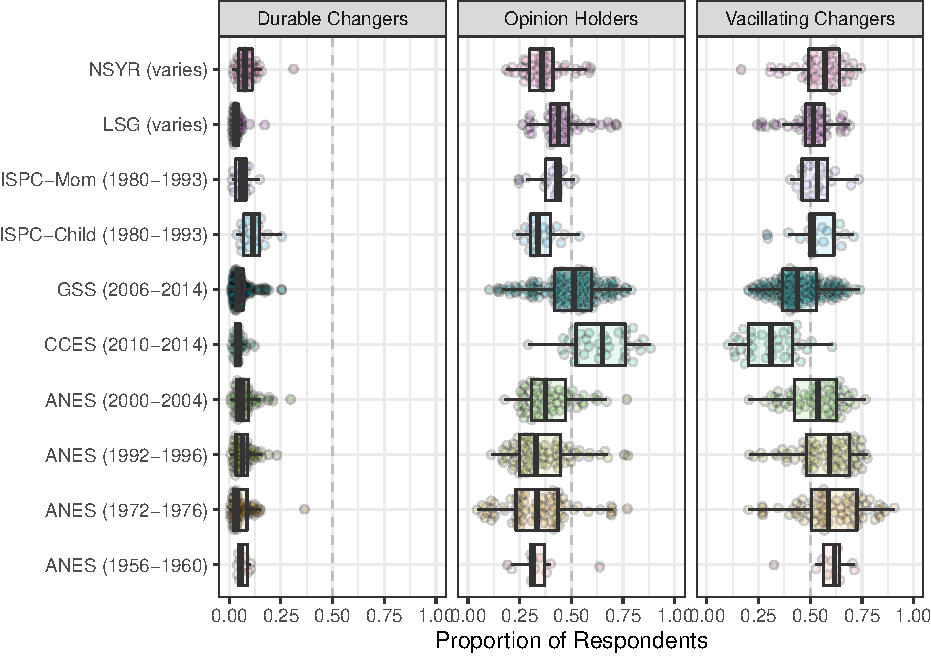
\includegraphics{ambivalence_everywhere_files/figure-latex/patterncomp-1.pdf}
\caption{\label{fig:patterncomp}Mean proportion of respondents in each behavioral group, by question and data set. Posterior distribution estimated with 5 chains, 2500 iterations each, first 500 iterations of each chain discarded.}
\end{figure}

Starting at the left, durable change is rare across all data sets and almost all questions. Consistent with Hypothesis 2, for about half of all questions, the mean estimated proportion of respondents demonstrating durable change is less than 5 percent, with many of these questions showing rates indistinguishable from 0.\footnote{Because of the conservative nature of the estimation process, the estimate for the proportion of durable changers can never be 0. But most of these questions have confidence intervals that extend below 1 percent and many iterations for these questions assign no respondents to the durable change group.} Only 17 percent of questions have mean rates of durable change above 10 percent. Attitudes that exhibit high levels of durable change typically pertain to high-profile public issues, and they are exceptions that prove the rule that durable change is, in general, rare.

Most of the data sets analyzed here include questions that demonstrate both high (greater than 70 percent) and low (less than 30 percent) levels of stability and vacillation. Since within-survey comparisons reflect the same sample, vacillation is not a feature of the population (the kinds of people being surveyed) but an interaction between people taking the survey and the kind of question being asked. In other words, there are some questions that most of the sample gives clear opinions over time, and there are questions on which very few people in the sample articulate clear opinions over time. However, most questions fall somewhere in the middle, with some people answering consistently and others not. This provides broad support for Hypothesis 1.

Third, consistent with Hypothesis 3, the vacillating changer group tends to be larger than the opinion holder group for most of the questions analyzed. The 1956-60 ANES panel, which Converse analyzed to generate his original insights about non-attitudes, displays the highest average level of vacillation, but it is not an outlier. Almost all surveys include questions that surpass that average estimate of ambivalence. The GSS and the CCES are the only data sets where more questions show higher levels of stability than vacillation.

Figure \ref{fig:strongcomp} plots the proportion of opinion holders and vacillating changes who give strong responses, conditional on them expressing an opinion (not saying ``no opinion''/``neither agree nor disagree''), for questions with four, five, or seven response options. Questions with two and three response options are excluded here as they lack ``strong'' responses. Points above the line indicate questions where opinion holders give ``strong'' responses at a higher rate than vacillating changers, conditional on giving an opinion.

\begin{figure}
\centering
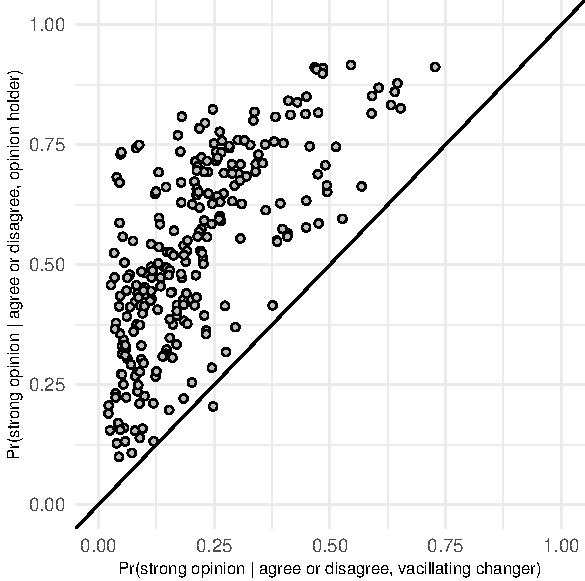
\includegraphics{ambivalence_everywhere_files/figure-latex/strongcomp-1.pdf}
\caption{\label{fig:strongcomp}Mean estimated proportion of ``strong'' responses in opinion holder and vacillating changer behavioral group. Posterior distribution estimated with 5 chains, 2500 iterations each, first 500 iterations of each chain discarded.}
\end{figure}

Opinion holders are more likely than vacillating changers attitudes to respond with a strong position, often much more likely. Vacillating changers tend to say that their opinions are weak and, as we would expect of weak opinions, switch sides of the scale. At the same time, vacillating changers still select the ``strong'' option, often quite frequently, suggesting that they tend to have a larger response range than opinion holders.

Figure \ref{fig:sdcomp} presents two sets of plots that compare the mean estimate of average within-person standard deviations for different behavioral groups. The top row compares vacillating changers to durable changers, and the bottom row compares vacillating changers to opinion holders. Because opinion holders always have a within-person standard deviation of 0 on questions with 2 or 3 response options, these questions are omitted. Points below the solid diagonal line indicate questions where the vacillating changers have greater within-person variance than the comparison group (durable changers in the top row, opinion holders in the bottom).

\begin{figure}
\centering
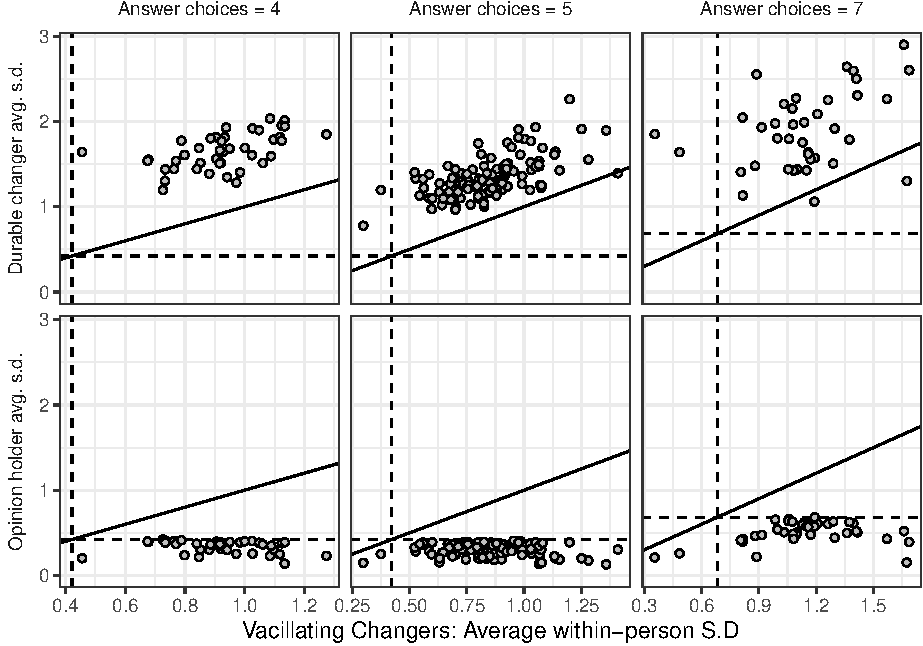
\includegraphics{ambivalence_everywhere_files/figure-latex/sdcomp-1.pdf}
\caption{\label{fig:sdcomp}Average within-person standard deviation, by behavioral group and question response options. Solid black line indicates equal within-group standard deviations. Dashed line indicates largest average within-person standard deviation for stable opinion holders. Posterior distribution estimated with 5 chains, 2500 iterations each, first 500 iterations of each chain discarded.}
\end{figure}

Consistent with the gay marriage example presented above, vacillating changers uniformly have higher within-person standard deviations than opinion holders for questions with four or more response options, regardless of question structure, and almost uniformly lower within-person standard deviations than durable changers.\footnote{The three questions where durable changes have lower average within-person standard deviation than vacillating changers ask respondents if if the government should bus students to ensure racial equality (72-76 ANES), whether the government should do more to improve the conditions of blacks (92-96 ANES), and whether they are happy with their bodies (NSYR).} Durable changers appear to move from one strong attitude to another while vacillating changers cluster in the middle of the scale. In other words, we can be fairly confident the model is separating three different groups with distinct sets of opinion behavior.

As an overall conclusion, the model detects three distinct sets of behavior, consistent with Converse's original black and white model, with the addition of a durable change group. Opinion holders exhibit strong opinions at the ends of scales. Vacillating changers have a much wider range of responses that vacillate on either side of the issue. Durable changers move between ends of the scale, often from one extreme to another. While we can say that overall, durable change is rare, there is a large variance in stability and vacillating change that remains to be explained.

It is difficult just looking at the overall patterns to say whether question content or structure drives overall rates of stability or vacillation. The GSS has more questions with fewer response options (questions with two, three, or four choices make up most of the GSS questions), but also more questions about non-political content. ANES questions tend to have more response options but focus almost exclusively on politics. Appendix B outlines a regression approach to evaluate the competing influences of structure and content on attitude stability and change.

Structure and content explain about 50 percent of the variation in rates of vacillation. Questions with fewer response options show higher stability, net of question content. Questions about sex and religion show slightly higher rates of stability than questions about politics, and questions about general morality and civil liberties show higher rates of vacillation than other questions, net of question structure. Questions about race, foreign relations, work, crime, and family and gender are not more or less stable than general political questions once I account for question structure.

There are some questions that are poorly explained by these tags. Across data sets, partisan identification is more stable than other measures of general political ideology (position on liberal-conservative scale; role of government in economy; role of government in equal opportunity, etc.). Questions about specifics -- specific policies and specific behaviors -- tend to be more stable than predicted while questions about general concepts (ideology, broad morality, etc.) tend to vacillate more than predicted.

Content explains less variation in rates of durable change, and there is no clear pattern in terms of question structure. The NSYR and the child panel of the ISPC, the two panels with with youngest average age, show higher rates of durable change than other panels, even controlling for questions structure and content. The largest residual in the durable change model pertains to people's evaluation of Richard Nixon in the 1972 to 1976 ANES panel, in which a large proportion of people shifted from a positive opinion or no opinion to a negative opinion. Given that this window covers from Nixon's victory in the 1972 election through the Watergate scandal and his eventual resignation, this shift is not surprising.

\hypertarget{issue-publics}{%
\subsection{Issue Publics}\label{issue-publics}}

The 166 questions in the GSS panels examined here produce 13,695 pairwise correlations.\footnote{There are seven federal spending questions where different versions are tested for different people, examined separately above. The two versions show minimal differences, so I consolidate each pair into a single item for this analysis.} In general, pairwise correlations between rates of stability are very low, with an average correlation of .04, suggesting stability in one attitude is not a strong predictor of stability in another attitude and that stability is not a function of the person answering the question. At the same time, some pairwise correlations are quite strong. To better understand the distribution of these strong correlations, I plot them as a network diagram in Figure \ref{fig:stabgraph}. For parsimony, I focus on the 541 correlations where \(\rho > .2\), about 2 percent of all correlations. Ties between issues indicate that people who are stable on one issue are stable on the other, and that people who vacillate on one issue vacillate on the other. The 58 questions with no \(\rho > .2\) are held out of the figure. The isolates include a heterogeneous mix of questions about gun laws, whether there is an afterlife, whether premarital sex is acceptable, and more.

\begin{figure}
\centering
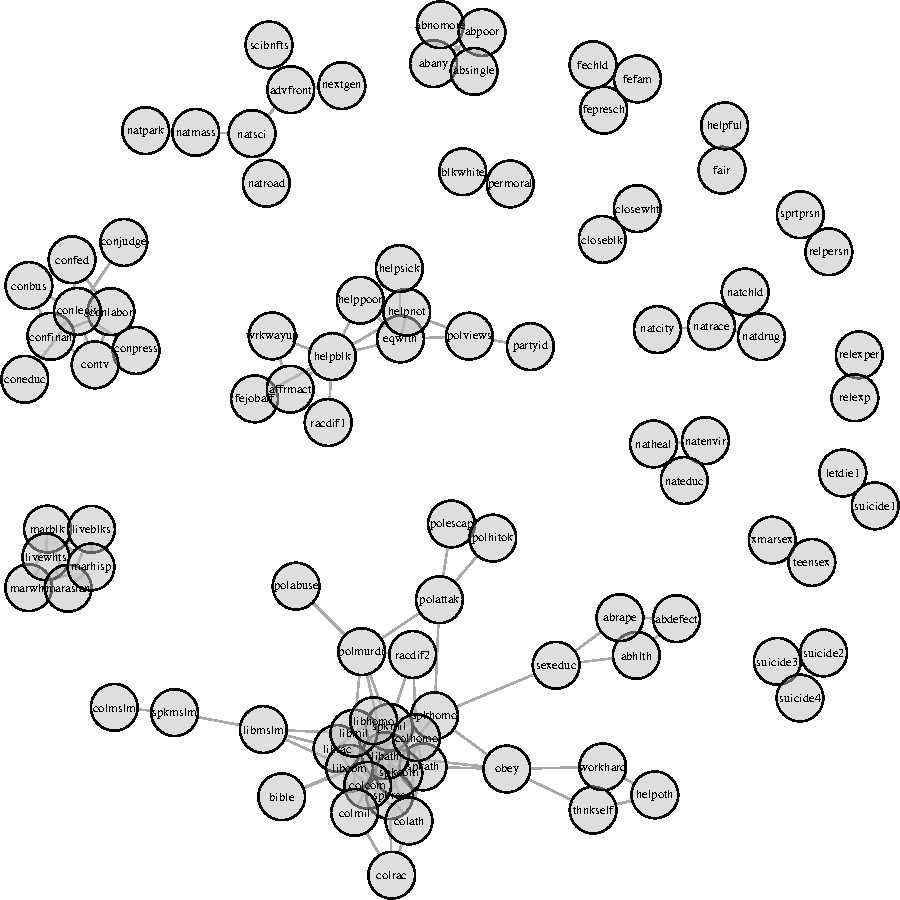
\includegraphics{ambivalence_everywhere_files/figure-latex/stabgraph-1.pdf}
\caption{\label{fig:stabgraph}Network graph of pairwise correlations of co-occuring stability greater than .2. Probabilities generated from group assignments over 10,000 draws from posterior distribution.}
\end{figure}

Figure \ref{fig:stabgraph} reinforces the ``issue public'' nature of attitude stability, showing a series of disparate attitude clusters. Substantively related issues tend to demonstrate simultaneous stability. The largest component of the network is a dense cluster of questions about civil liberties (colath, libhomo, spkrac, etc.), that spans out to questions of police use of force (polhitok), abortion (abhlth), and the values that should be demonstrated by children (obey, helpoth). These questions tend to reflect the application of general standards across specific instances, and preliminary analysis suggests that higher levels of education is associated with stability on issues in this cluster. This component is disconnected from a second large cluster about political views, including ideology (polviews), partisan identification (partyid), and views on government and race (helpblk, affact). Other ``issue publics'' connect issues on government spending priorities (natcity, natrace, natdrug), confidence in institutions (conlegis, coneduc), beliefs about gender (fefam, fepresch), and beliefs about science (advfront, natci).

Notable in the figure are the lack of connections between certain issues. Despite having a similar structure and appearing next to each other in the survey, two sets of questions about abortion are disconnected -- holding a stable belief about abortion in some circumstances (child defect, women's health, and rape) is not related to a stable position on abortion in other circumstances (single mother, as a method of birth control, if the mother is poor, and any circumstance the woman wants). The same is true of beliefs about euthanasia and suicide. Stability in general political beliefs (liberal-conservative ideology, partisan identification) is disconnected from a broad set of questions about government spending. Questions about generalized trust are disconnected from specific questions about confidence in institutional leadership, and questions about specific morality are disconnected from questions about general morality.

\hypertarget{discussion}{%
\section{Discussion}\label{discussion}}

The results presented above suggest several conclusions about the behavior of attitudes, at least the attitudes that get measured in social science surveys. First, it is wrong to say that people do not hold durable opinions. On most issues, there is some proportion of the population that consistently locates itself on one side of an issue or another in ways that cannot be attributed to chance. When people hold opinions stably, they are disproportionately likely to say they hold this opinion strongly, a finding consistent with psychological models of strong attitudes (Howe and Krosnick 2017). While simpler questions -- those with fewer answer choices or less abstract wording -- seem easier for people to answer consistently over time, some proportion maintain stable attitudes even on complicated, abstract, conceptual questions.

At the same time, it is wrong to say that people in general ``have'' opinions. There is typically a large group of people who do not maintain consistent opinions on any particular issue, vacillating between ends of the scale and in their extremity in ways that suggest they are subject to short-term considerations. Differences in the average within-person standard deviations for opinion behavior groups suggests people who vacillate are not just people at the middle of the scale who report with error; they often span the scale. These patterns are strongly consistent with Zaller's notion of ambivalence, that on any particular issue, ``people are likely to internalize many contradictory arguments'' and ``form considerations that induce them both to favor and oppose the same issues'' (1992: p.~59). This is true not just of politics, but also of general morality, opinions about racial issues, evaluations of public figures and groups, and more.

With the exception of questions about religious beliefs and sex, people were not more likely to be consistent on non-political issues than political issues. While questions about political issues demonstrate high levels of ambivalence, they are not unique in that regard. People are ambivalent about morality, civil liberties, race, gender, family structures, medicine, and more. In fact, when issues in other domains -- race, social trust, medicine, etc. -- interact with the political space, people seem more likely to report the same opinion consistently. This suggests, consistent with Zaller's model and studies of cognitive authorities, that people get their cues about what to believe from opinion leaders, regardless of domain (Martin 2002; Rawlings 2020; Zaller 1992).

Across domains, specific attitudes tend to be more stable than general attitudes. People are more likely to be consistent on specific moral prohibitions than on general questions about morality. They are more stable on specific questions about government spending on various priorities than on general questions about the role of government and political ideology. This suggests people work inductively from specifics to general principles and have a hard time reconciling disparate specifics. They do not seem to apply general principles to specific outcomes. In the political domain, this is consistent with the notion that people are ``ideologically innocent'' (Kinder and Kalmoe 2017) and further argues against general or latent beliefs. This, combined with the fact that issues demonstrate greater stability when they intersect with the political realm, suggests stability on issues is a function of what people hear, with specific issues more frequently discussed than general principles.

\hypertarget{implications-for-cultural-sociology}{%
\subsection{Implications for Cultural Sociology}\label{implications-for-cultural-sociology}}

For cultural sociology, the results presented here reinforce notions that opinion stability is a function of social scaffolding -- institutions, contexts, and social networks (Lizardo and Strand 2010; Martin 2002). Exactly what kinds of social scaffolding, and where in the life course these influence matters most, is unclear from these results, though young people appear to be making more durable change than older people, suggesting they are more susceptible to environmental influences. It could be the case that people with stable dispositions acquire these early in life, while people who do not acquire these early never do. It could also be the case that people who hold stable attitudes do so because they are embedded in social structures that facilitate them. Adjudicating the mechanisms that facilitate stability requires further work that can be facilitated by adding group-predicting parameters to the finite mixture model.

The low proportions of people making durable change reinforce the recent finding that people have relatively stable views by the time they reach adulthood (Kiley and Vaisey 2020; Vaisey and Lizardo 2016). Higher rates of durable change in the NSYR and the child panel of the ISPC -- especially compared to the mother panel that asks the same questions and extends of the same time -- suggest young people are more susceptible to social influences than older people. At the same time, high vacillation or ambivalence in many questions challenges the finding that adults have ``settled dispositions.'' Many survey respondents agree with a statement in one wave and disagree in another. While we can say that large swaths of the population have settled dispositions on questions about sexual morality, religious beliefs, and some specific governmental policies, they lack consistent opinions on more general conceptual questions -- political ideology, general beliefs about the role of government, general morality, and abstractions about civil liberties. If people tend to be ambivalent, then it is possible for their attitudes to be influenced by a consolidation of elite opinion around a topic. However, so long as culture remains heterogeneous, it seems likely that large groups of the population will vacillate.

These results suggest a high proportion of the population is subject to short-term influences, but that these influnces have little durability over time. They reinforce the idea that the heterogeneity of cultural considerations in the public sphere cause people to contradict themselves over time, not just in interviews but in survey measures as well (Swidler 2001).

\hypertarget{implications-for-measuring-attitudes}{%
\subsection{Implications for Measuring Attitudes}\label{implications-for-measuring-attitudes}}

Measurement error theories suggest that over-time variance in survey responses over time is principally a function of question structure, but these theories struggle to find features of attitude questions that explain of this variation (Alwin 2007). The results presented here reinforce findings in public opinion research that instability is an interaction of the question and the person answering the question (Freeder, Lenz, and Turney 2019; Zaller 1992). If variation in responses over time principally reflects the heterogeneity of considerations people carry with them, then measuring attitudes over time might be a way to understand the bredth of considerations people surface over time.

Researchers invoke the weak but present predictive power of attitudes to argue both for and against a link between attitudes and behaviors (Jerolmack and Khan 2014; Vaisey 2014). The prevalence of weak attitudes -- inconsistency that seemingly cannot be attributed to measurement error -- should caution researchers away from assuming that cross-sectional measures of attitudes are a good proxy for an underlying belief. For many questions, more than half a sample might be responding with a temporary attitude construct, while others report real attitudes that matter to them. Given this heterogeneity, we should not expect strong predictive ability for an attitude in general, but that tells us nothing about how it influences the people for whom the attitude does matter. ``Attitude effects'' are going to be shaped by what proportion of the population finds an attitude to be meaningful, the distribution of stable attitude holders in the population, and the actual effect of the attitude on behavior. At the same time, it is not clear how many respondents need to be making stable responses for an attitude to be a good predictor for behavior (a coarsened version of the question Vaisey (2009) used to predict behavior was only stable for about 27 percent of respondents).

\hypertarget{conclusions}{%
\section{Conclusions}\label{conclusions}}

This paper sought to clarify a divide in both cultural sociology and public opinion scholarship between theories suggesting that people lack clear opinions and those suggesting that people hold stable, real opinions. Going back to Converse's original formulation of the ``black and white'' model, I suggested that for any particular question, both were likely true: some people hold real, stable attitudes while other people draw on disparate considerations to construct a new opinion each time they are asked. Using a finite mixture model with three theoretically grounded models of opinion behavior, I quantified the proportion of survey respondents who held stable opinions, those who vacillated or gave ambivalent responses, and those who formed an opinion or changed their opinion during the course of the survey. The vacillating group tended to outnumber opinion holders. This set of results is consistent with Zaller's model of ambivalence, but also suggests that some people in the population do form stable, real opinions in certain circumstances.

Ultimately, these results suggest that researchers should devote attention to the social conditions that facilitate stable attitudes and dispositions, whether they are located in people's past or in their contemporary environment. While we know that political awareness tends to facilitate stability in political beliefs, we have no expectation that political awareness should facilitate stability beliefs about religion, morality, or more, but it does suggest that domain-specific awareness might predict domain-specific stability. Attention to the mechanisms that create attitudes can help researchers develop a better understanding of the role of culture in behavior.

\hypertarget{appendix-a-model-estimation}{%
\section{Appendix A: Model Estimation}\label{appendix-a-model-estimation}}

The following is a summary of the model used here, outlined in Hill and Kreisi (Hill and Kriesi 2001b), with modifications for three waves rather than the four they use in their analysis. Comparing a four-wave model to a three-wave model using data from the NSYR and LSG, which have more than three waves, to a model with the same data, dropping an interior wave (wave 2 or 3), produces comparable estimates for most coefficients, especially behavioral group proportions (\(\pi_1\), \(\pi_2\), and \(\pi_3\)), suggesting the model behaves just as well with three waves.

The goal of the Data Augmentation algorithm is to draw a plausible set of parameters, \(p(\theta|Z)\), compatible with the observed data (\(Z\)) and the assumptions made in the model. It iterates through two main steps: Drawing group membership indicators, given the parameter, and drawing parameters given the group membership indicators. I first outline the variables that go into the model and then outline those steps below.

\hypertarget{re-expressing-the-data}{%
\subsection{Re-Expressing the Data}\label{re-expressing-the-data}}

Rather than estimate parameters on the basis of full patterns, such as ``agree''-``disagree''-``strongly disagree,'' I characterize a respondent by a set of general variables. These variables retain the features of the data without having to generate a probability for each pattern separately. For example, by re-expressing the data in this manner I collapse the distinction between someone who says ``agree''-``strongly agree''-``agree'' and someone who says ``agree''-``agree''-``strongly agree.'' Both patterns become someone who remains on the same side of an issue and gives one strong response.

\begin{align*}
A_i&=\begin{cases}
  1 & \text{is the }i\text{th person's initial response is a 4 or 5}\\
  0 & \text{otherwise}\\
  \end{cases} \\
B_i&=\text{number of the }i\text{th individual's responses that are either 1 or 5 across all } t \\
C_i&=\text{number of the }i\text{th individual's responses that are 3} \\
D_i&=\text{number of times the }i\text{th individual crosses an opinion boundary} \\
E_i&=\begin{cases}
  0 & \text{if } D_i \neq 1\\
  t_i^* & \text{otherwise}\\
  \end{cases} \\
F_i&=\begin{cases}
  0 & \text{if the }i\text{th individual's preswitch response is a 1, 2, or 3, or } D_i \neq 1\\
  1 & \text{if the }i\text{th individual's preswitch response is a 4 or 5}\\
  \end{cases} \\
H_i&=\begin{cases}
  0 & \text{if the }i\text{th individual's preswitch response is a 1, 2, 4, or 5, or } D_i \neq 1\\
  1 & \text{if the }i\text{th individual's preswitch response is a 3}\\
  \end{cases} \\
M_i&=\begin{cases}
  0 & \text{if the }i\text{th individual's postswitch response is a 1, 2, or 3, or } D_i \neq 1\\
  1 & \text{if the }i\text{th individual's postswitch response is a 4 or 5}\\
  \end{cases} \\
Q_i&=\begin{cases}
  0 & \text{if the }i\text{th individual's postswitch response is a 1, 2, 4, or 5, or } D_i \neq 1\\
  1 & \text{if the }i\text{th individual's postswitch response is a 3}\\
  \end{cases} \\
R_i&=\text{number of the }i\text{th individual's responses that are either 1 or 2 across all } t \\
\end{align*}

I denote the vector of these random variables for individual i as \(Z_i\). For the seven-point scale, I include an additional variable that counts ``weak'' responses.

\hypertarget{drawing-group-indicators-given-parameters}{%
\subsection{Drawing Group Indicators Given Parameters}\label{drawing-group-indicators-given-parameters}}

I use the observed data \(Z_i\) and parameter estimates to determine the probability that a person falls into each behavioral group. The conditional probability of belonging to each behavior group given the observed responses and estimated parameters is expressed by the following functions:

\begin{align*}
p_{1,i}^z& =(\alpha_i^{(1-A_i)}(1-\alpha_1)^{A_i}(1-\delta_1)^{(3-B_i)}\delta_1^{B_i})I(C_i=0)I(D_i=0) \\
p_{2,i}^z& =\varphi_2^{C_i}\alpha_2^{R_i}(1-\varphi_2-\alpha_2)^{(3-C_i-R_i)}\delta_2^{B_i}(1-\delta_2)^{(3-C_i-B_i)} \\
p_{3,i}^z& =[\tau_3^{I_{(E_i=1)}}(1-\tau_3)^{I_{(E_i=2)}}({\varphi_3^{(pre1)}}^{H_i}{\alpha_3^{(pre1)}}^{(1-F_i)(1-H_i)}(1-\alpha_3^{(pre1)}-\varphi_3^{(pre1)})^{F_i})^{I_{(E_i=1)}} \\
&   \times ({\varphi_3^{(pre2)}}^{H_i}{\alpha_3^{(pre2)}}^{(1-F_i)(1-H_i)}(1-\alpha_3^{(pre2)}-\varphi_3^{(pre2)})^{F_i})^{I_{(E_i=2)}} \\
&   \times ((1-\alpha_3^{(post)})^{M_i}(\alpha_3^{(post)})^{(1-M_i)})^{H_i}\delta_3^{B_i}(1-\delta_3)^{(3-C_i-B_i)}]I(D_i=1)I(Q_i=0) \\
\end{align*}

where \(I(.)\) equals 1 if the condition in the parentheses is met and 0 otherwise. These probabilities represent the expected frequency of a particular pattern given the parameters that describe behavior in that opinion behavior group. For example, if a person responds ``no opinion'' or ``neither agree nor disagree'' in one wave, then \(D_i \neq 0\), and \(p_{1,i}^z\) will equal 0 for that person, since people who express ``no opinion'' can not be opinion holders. If \(\alpha_1=.5\) and \(\delta_1=.75\), we expect patterns where a person give a ``strongly disagree'' response in all three waves to make up about 21 percent of responses in group 1.

Generating these probabilities requires parameter estimates. In the first iteration of the model, these parameters are drawn at random from the parameter space. These random draws are only bound by logical constraints, such as proportions summing to 1.

With these probabilities and draws for \(\pi_1\), \(\pi_2\), and \(\pi_3\) (sampled randomly from the parameter space in the first iteration), I sample from the following trinomial distribution for each person to generate group membership indicators for each iteration.

\begin{equation}
p(G_i|\theta,Z_i)=\text{Mult}\left(\frac{\pi_1p_{1,i}^z}{\sum_{j=1}^3\pi_jp_{j,i}^z},\frac{\pi_2p_{2,i}^z}{\sum_{j=1}^3\pi_jp_{j,i}^z},\frac{\pi_3p_{3,i}^z}{\sum_{j=1}^3\pi_jp_{j,i}^z}\right)
\end{equation}

These draws generate group membership indicators for a single iteration of the model. The probability that a person's responses are generated from a particular pattern are a function of the likelihood that a pattern was generated by a particular behavioral group, \(p_{i,j}\), and the overall prevalence of that behavioral group in the population, \(\pi_j\). While a pattern ``strongly agree''-``agree''-``strongly agree'' might be most consistent with a stable opinion, as the proportion of the population vacillating changers increases, the probability that the vacillating group produced this pattern increases as well. While it is unlikely (Probability = 0.001) that someone behaving consistent with the vacillating changer group in the gay marriage example would give three ``strongly agree'' responses, the probability we observe someone doing that is much larger if the group is 1,000 people rather than 10.

\hypertarget{drawing-parameters-given-group-indicators}{%
\subsection{Drawing Parameters Given Group Indicators}\label{drawing-parameters-given-group-indicators}}

With group memberships temporarily assigned for one iteration, I then draw parameter estimates from their distribution conditioning on the data (\(Z_i\)) and the group indicators. In other words, I fit separate models for each (temporarily assigned) behavioral group to generate parameter estimates for that iteration.

I use Beta and Dirichlet distributions for prior distributions for each parameter. Assuming a priori independence of the appropriate parameters, I factor \(p(\theta)\) into six independent Beta distributions -- \(p(\alpha_1, 1-\alpha_1)\), \(p(\delta_1, 1-\delta_1)\), \(p(\delta_2, 1-\delta_2)\), \(p(\alpha_3^{(post)}, 1-\alpha_3^{(post)})\), \(p(\delta_3, 1-\delta_3)\), \(p(\tau_3, 1-\tau_3)\) -- and four independent Dirichlet distributions -- \(p(\varphi_2, \alpha_2, 1-\varphi_2-\alpha_2)\), \(p(\varphi_3^{(pre1)}, \alpha_3^{(pre1)}, 1-\varphi_3^{(pre1)}-\alpha_3^{(pre1)})\), \(p(\varphi_3^{(pre2)}, \alpha_3^{(pre2)}, 1-\varphi_3^{(pre2)}-\alpha_3^{(pre2)})\), \(p(\pi_1, \pi_2, \pi_3)\).\footnote{In the seven-point-scale model, \(\delta\) and \(\gamma\) estimates are drawn from a Dirichlet distribution (one for each behavioral group), rather than the Beta distribution for the \(\delta\) estimate in the five-point-scale model. In the three-point-scale model, no \(\delta\) parameter is estimated.} Parameters are then drawn from the appropriate posterior distributions, using only people in that particular behavioral group. These posterior distributions amount to summing up people or responses that demonstrate that behavior and adding the relevant prior to the count. For example, the posterior distributions for the three \(\pi_j\) parameters and the two group 1 behaviors are:

\begin{align*}
p(\pi_1, \pi_2, \pi_3)&=\text{Dirichlet}[(\sum_{i=1}^N G_i=1 + 2), (\sum_{i=1}^N G_i=2 + 2), (\sum_{i=1}^N G_i=3 + 2)] \\
p(\alpha_1, 1-\alpha_1)&=\text{Beta}[(N - \sum_{i=1}^N A_i + 1), (\sum_{i=1}^N A_i + 1)] \\
p(\delta_1, 1-\delta_1)&=\text{Beta}[(\frac{\sum_{i=1}^N B_i}{3} + 1), (N - \frac{\sum_{i=1}^N B_i}{3} + 1)] \\
\end{align*}

The formulas look complicated, but they amount to counting the number of response patterns that follow the particular rule the parameter pertains to. This is most obvious in the case of the \(\pi_j\) estimates, which are a Dirichlet draw from the count of each person assigned to that group for the current iteration, plus two additional cases in each group (the prior). Similarly, the estimate for \(\alpha_1\), \((N - \sum_{i=1}^N A_i + 1)\), is simply the total number of people in Group 1 (opinion holders), \(N\), minus the number of people who disagree, \(\sum_{i=1}^N A_i\), plus 1 (the prior). Since opinion holders can only agree or disagree, this gives the count of people who agree, which is what \(\alpha_1\) indicates.

As noted above the priors are functionally equivalent to adding two people to each behavior group and splitting up their behavior within those groups. Hill and Kreisi find that changes in these priors have minimal effects on the actual estimates. The greatest instability is observed in the durable changers group, which is often small and therefore more susceptible to the influence of priors.

\hypertarget{convergence}{%
\subsection{Convergence}\label{convergence}}

To percent the randomly drawn starting values to unduly influence the parameter estimates, I draw five different sets of starting parameters for each question. The model iterates until these five chains reach a stable distribution, from which draws were taken to capture the posterior distribution. Functionally, I used five chains, each with 2500 iterations. I discarded the first 500 iterations to eliminate estimates generated prior to convergence. Diagnostics suggest that, for most questions, parameter estimates converged well before the 500th iteration.

These posterior distributions are then summarized.

\hypertarget{appendix-b-question-content-and-structure}{%
\section{Appendix B: Question Content and Structure}\label{appendix-b-question-content-and-structure}}

To better assess the influence of question content and structure, I tagged questions with broad indicators for content areas: government and politics; civil liberties; medicine and science; race; sex; family and gender\footnote{Ideally I would include separate indicators for questions relating to gender and questions relating to family structures. However, almost all questions about gender touch on some other subject material, with family structures being the largest overlap.}; socioeconomic position; work; morality; foreign relations; self-evaluations; religion; crime; social trust; and other. These categories are not mutually exclusive, and many questions are asked in a survey because feature the intersection of multiple domains. Because of this, I focus on an explicit reading of the question and code items parsimoniously. Because more than half of all questions analyzed here touch on government and politics in some capacity, I instead use an indicator to signal that a question does \emph{not} explicitly deal with politics. I also include indicators for whether a question asks people to assess another person's position, and indicators for whether the question refers to a clear group of people or a particular person.

I also create indicator variables for question structure. First, I include five indicators about question format. The first format asks whether people agree with a statement. These include traditional five- and four-point Likert scales and two- and three-point agree/disagree or yes/no statements. The second format asks people to select a position select between two poles or options. The third format, common in the ANES panels, asks respondents to place a respondent on a ``feeling thermometer.'' A fourth format asks people whether groups have ``too much'' influence in politics. The final category includes other question structures. Most questions in this last category evaluate the intensity of something, such as whether an amount should increase, stay the same, or decrease. While many questions with ``other'' structures were collapsed to reflect a ``yes/no'' structure, I code based on the original wording. I also include indicator variables for the number of response options (2, 3, 4, 5, 7) and indicator variables for data set.

I then regress the proportion of respondents falling into each behavioral group on these indicators. As noted above, the questions explored here do not represent a random sample of questions, so standard confidence intervals and statistical inferences are not meaningful. However, I incorporate uncertainty in two ways. First, I bootstrap coefficient estimates, randomly sampling questions with replacement 10,000 times. Second, to incorporate the uncertainty in each question's proportion estimate, each time a parameter is sampled in the bootstrap, I draw a random value from that parameter's posterior distribution. By bootstrapping the estimates I can be relatively confident that whatever patterns I observe are not driven by a single question or small group of questions with unusual behavior, even if I cannot generalize to all attitudes.

In all regressions, the reference group consists of general questions about government (particularly government's role in the domestic economy) on a five-point agree/disagree scale, with the General Social Survey serving as the reference data set.

\hypertarget{vacillation}{%
\subsection{Vacillation}\label{vacillation}}

Figure \ref{fig:vacboot} presents coefficient estimates for a regression of the proportion of respondents giving vacillating response patterns on question content and structure. An unpictured regression of the proportion of respondents giving durable change response patterns on the same parameters is almost a mirror-image of the figure presented here, with the variables predicting higher vacillation predicting lower stability. As a result, I will discuss both stability and vacillation in reference to the Figure \ref{fig:vacboot}.

\begin{figure}
\centering
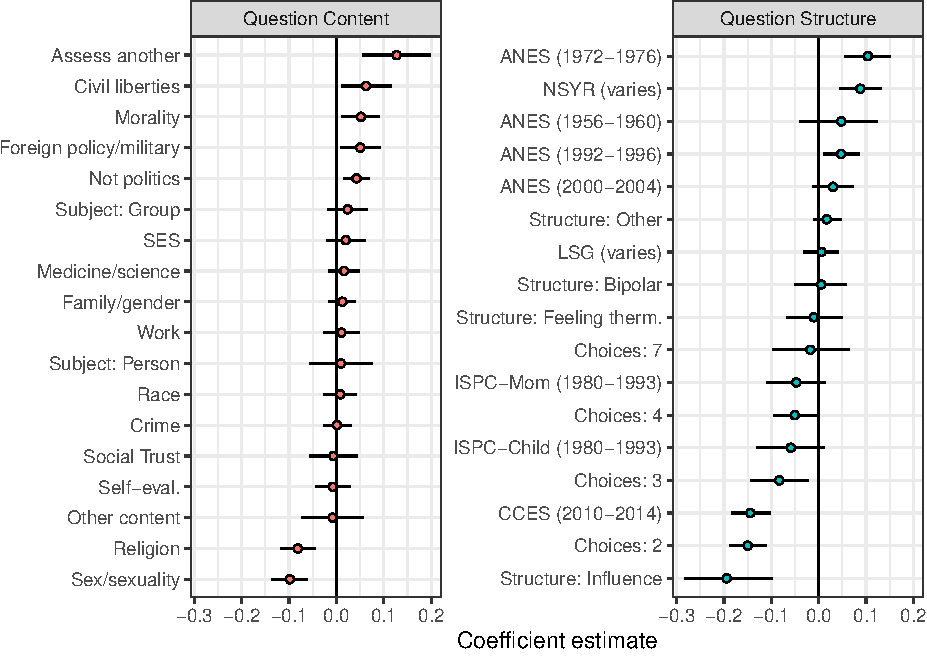
\includegraphics{ambivalence_everywhere_files/figure-latex/vacboot-1.pdf}
\caption{\label{fig:vacboot}Coefficient estimates of regression of proportion of respondents of giving a vacillating response on question content and structure indictors. Confidence intervals generated from 10,000-iteration bootstrap.}
\end{figure}

A general five-point agree/disagree question about domestic government and politics from the GSS has an expected proportion of people vacillating of about .58 with a standard error of .033. Two content areas demonstrate notably less vacillation than other kinds of questions: questions about religious beliefs and questions about sex and homosexuality. On the other end of the scale, questions about general morality, questions about civil liberties, and questions about medicine and science show more vacillation than other kinds of questions. When questions fall outside of the political space (``Not politics'' in Figure \ref{fig:vacboot}), they tend to show higher levels of vacillation. Notably, questions about race, foreign relations, work, crime, and family and gender do not appear substantially different from questions about politics once I control for question structure.

Questions that ask people to assess others -- where do politicians or parties fall on particular issue scales -- demonstrate much higher vacillation than questions about people's own opinions. This is consistent with previous work (Alwin 2007) and suggests a lack of knowledge about actors' in the political sphere.

In terms of question structure, stability decreases and vacillation increases as the number of response options increases. This helps explain the higher levels of stability for GSS and CCES questions, which have fewer response options on average, relative to the other data sets. Questions about groups' political influence show more stability than other kinds of questions, but beyond that, question structure does not seem to matter much.

Finally, even controlling for question structure, data sets demonstrate different rates of vacillation. Notably, the 1972-1976 ANES and the NSYR demonstrate more vacillation than other data sets. The CCES demonstrates lower rates of vacillation.

\hypertarget{durable-change}{%
\subsubsection{Durable Change}\label{durable-change}}

Figure \ref{fig:durableboot} plots coefficient estimates of the proportion of respondents demonstrating durable change. The coefficients associated with question content and structure are much smaller on durable change than on vacillating change, reflecting its truncation in low end of the proportion rage, and the parameters here do not explain nearly as much variance as the model for vacillating change. There is almost no appreciable effect of question content on the rate of durable change.

\begin{figure}
\centering
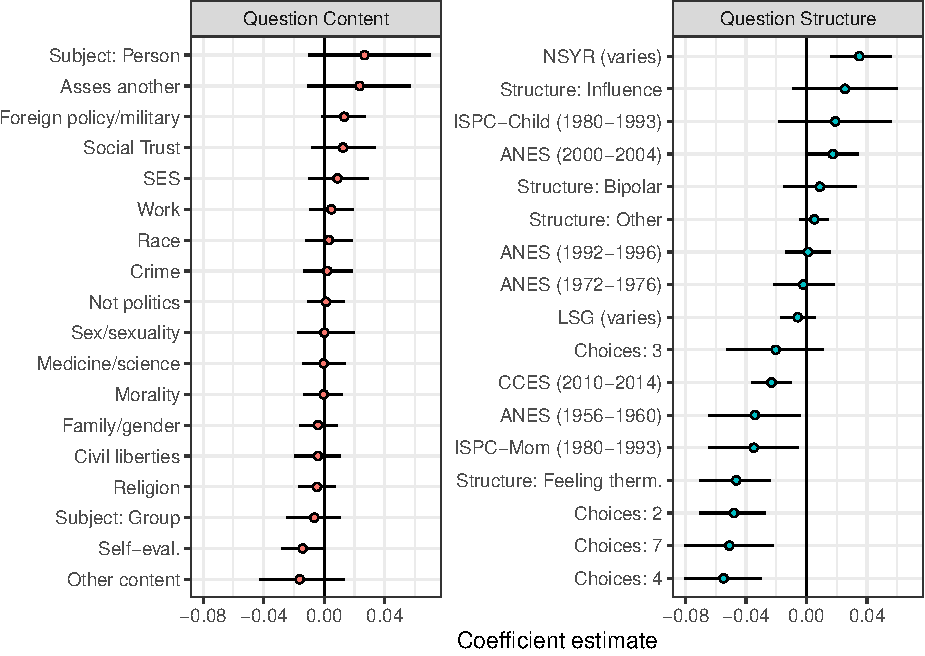
\includegraphics{ambivalence_everywhere_files/figure-latex/durableboot-1.pdf}
\caption{\label{fig:durableboot}Coefficient estimates of regression of proportion of respondents of giving a durable change response on question content and structure indictors. Confidence intervals generated from 10,000-iteration bootstrap.}
\end{figure}

Two data sets demonstrate substantially higher levels of durable change: the NSYR and the ISPC-Child, the two panels with the lowest average age.

There is a less clear pattern on question structure for durable change than for vacillating change. Questions with five response options (the reference category) demonstrate the most durable change, followed by questions with three responses. Questions with two, four, and seven responses demonstrate comparable, low levels of durable change.

In addition to the Nixon question discussed above, other questions with high rates of durable change include a shift in the NSYR in which many adolescents go from saying that people should wait to have sex until they are married to saying ``not necessarily,'' with very few shifting the other way, and a large change of opinion around whether the presidential election in 2000 was fair.

\newpage

\hypertarget{references}{%
\section{References}\label{references}}

\singlespace
\setlength{\parindent}{-0.2in}
\setlength{\leftskip}{0.2in}
\setlength{\parskip}{0pt}

\noindent

\hypertarget{refs}{}
\leavevmode\hypertarget{ref-achen1975}{}%
Achen, Christopher H. 1975. ``Mass Political Attitudes and the Survey Response.'' \emph{The American Political Science Review} 69 (4). {[}American Political Science Association, Cambridge University Press{]}: 1218--31. \url{https://doi.org/10.2307/1955282}.

\leavevmode\hypertarget{ref-alwin2007}{}%
Alwin, Alwin, Duane F. 2007. \emph{Margins of Error: A Study of Reliability in Survey Measurement}. Hoboken, N.J.: John Wiley \& Sons.

\leavevmode\hypertarget{ref-ansolabehere2008}{}%
Ansolabehere, Stephen, Jonathan Rodden, and James M. Snyder. 2008. ``The Strength of Issues: Using Multiple Measures to Gauge Preference Stability, Ideological Constraint, and Issue Voting.'' \emph{American Political Science Review} 102 (2): 215--32. \url{https://doi.org/10.1017/S0003055408080210}.

\leavevmode\hypertarget{ref-baker2004}{}%
Baker, Wayne. 2004. \emph{America's Crisis of Values: Reality and Perception}. Princeton, New Jersey: Princeton University Press.

\leavevmode\hypertarget{ref-baldassarri2008}{}%
Baldassarri, Delia, and Andrew Gelman. 2008. ``Partisans Without Constraint: Political Polarization and Trends in American Public Opinion.'' \emph{American Journal of Sociology} 114 (2): 408--46.

\leavevmode\hypertarget{ref-bellah1985}{}%
Bellah, Robert N., Richard Madsen, William M. Sullivan, Ann Swidler, and Steven M. Tipton. 1985. \emph{Habits of the Heart, with a New Preface}. Berkeley: University of California Press. \url{https://www.ucpress.edu/book/9780520254190/habits-of-the-heart-with-a-new-preface}.

\leavevmode\hypertarget{ref-converse1964}{}%
Converse, Philip E. 1964. ``The Nature of Belief Systems in Mass Publics (1964).'' In \emph{Ideology and Discontent}, edited by D. E. Apter, 18:206--61. New York: Free Press. \url{http://www.tandfonline.com/doi/abs/10.1080/08913810608443650}.

\leavevmode\hypertarget{ref-converse1979}{}%
Converse, Philip E., and Gregory B. Markus. 1979. ``Plus ca Change...: the New CPS Election Study Panel.'' \emph{The American Political Science Review} 73 (1). {[}American Political Science Association, Cambridge University Press{]}: 32--49. \url{https://doi.org/10.2307/1954729}.

\leavevmode\hypertarget{ref-dimaggio1997}{}%
DiMaggio, Paul. 1997. ``Culture and Cognition.'' \emph{Annual Review of Sociology} 23: 263--87.

\leavevmode\hypertarget{ref-erikson1979}{}%
Erikson, Robert S. 1979. ``The SRC Panel Data and Mass Political Attitudes.'' \emph{British Journal of Political Science} 9 (1). Cambridge University Press: 89--114.

\leavevmode\hypertarget{ref-freeder2019}{}%
Freeder, Sean, Gabriel S. Lenz, and Shad Turney. 2019. ``The Importance of Knowing `What Goes with What': Reinterpreting the Evidence on Policy Attitude Stability.'' \emph{The Journal of Politics} 81 (1): 274--90. \url{https://doi.org/10.1086/700005}.

\leavevmode\hypertarget{ref-gross2009}{}%
Gross, Neil. 2009. ``A Pragmatist Theory of Social Mechanisms.'' \emph{American Sociological Review} 74 (3). SAGE Publications Inc: 358--79. \url{https://doi.org/10.1177/000312240907400302}.

\leavevmode\hypertarget{ref-halpernmanners2012}{}%
Halpern-Manners, Andrew, and John Robert Warren. 2012. ``Panel Conditioning in Longitudinal Studies: Evidence from Labor Force Items in the Current Population Survey.'' \emph{Demography} 49 (4): 1499--1519. \url{https://doi.org/10.1007/s13524-012-0124-x}.

\leavevmode\hypertarget{ref-hill2001}{}%
Hill, Jennifer L. 2001. ``Accommodating Missing Data in Mixture Models for Classification by Opinion-Changing Behavior.'' \emph{Journal of Educational and Behavioral Statistics} 26 (2). American Educational Research Association: 233--68. \url{https://doi.org/10.3102/10769986026002233}.

\leavevmode\hypertarget{ref-hill2001a}{}%
Hill, Jennifer L., and Hanspeter Kriesi. 2001a. ``An Extension and Test of Converse's "Black-and-White" Model of Response Stability.'' \emph{The American Political Science Review} 95 (2). {[}American Political Science Association, Cambridge University Press{]}: 397--413.

\leavevmode\hypertarget{ref-hill2001b}{}%
---------. 2001b. ``Classification by Opinion-Changing Behavior: A Mixture Model Approach.'' \emph{Political Analysis} 9 (4). {[}Oxford University Press, Society for Political Methodology{]}: 301--24.

\leavevmode\hypertarget{ref-hout2016}{}%
Hout, Michael, and Orestes P. Hastings. 2016. ``Reliability of the Core Items in the General Social Survey: Estimates from the Three-Wave Panels, 2006--2014.'' \emph{Sociological Science} 3 (November): 971--1002. \url{https://doi.org/10.15195/v3.a43}.

\leavevmode\hypertarget{ref-howe2017}{}%
Howe, Lauren C., and Jon A. Krosnick. 2017. ``Attitude Strength.'' \emph{Annual Review of Psychology} 68 (1): 327--51. \url{https://doi.org/10.1146/annurev-psych-122414-033600}.

\leavevmode\hypertarget{ref-hunter2000}{}%
Hunter, James Davison. 2000. \emph{The Death of Character : Moral Education in an Age Without Good or Evil}. 1st ed. New York : Basic Books, c2000. \url{https://find.library.duke.edu/catalog/DUKE002791044}.

\leavevmode\hypertarget{ref-inglehart1985}{}%
Inglehart, Ronald. 1985. ``Aggregate Stability and Individual-Level Flux in Mass Belief Systems: The Level of Analysis Paradox.'' \emph{American Political Science Review} 79 (1): 97--116. \url{https://doi.org/10.2307/1956121}.

\leavevmode\hypertarget{ref-jerolmack2014}{}%
Jerolmack, Colin, and Shamus Khan. 2014. ``Talk Is Cheap: Ethnography and the Attitudinal Fallacy.'' \emph{Sociological Methods \& Research} 43 (2): 178--209. \url{https://doi.org/10.1177/0049124114523396}.

\leavevmode\hypertarget{ref-joas1996}{}%
Joas, Hans. 1996. \emph{The Creativity of Action}. Chicago: University of Chicago Press.

\leavevmode\hypertarget{ref-judd1980}{}%
Judd, Charles M., and Michael A. Milburn. 1980. ``The Structure of Attitude Systems in the General Public: Comparisons of a Structural Equation Model.'' \emph{American Sociological Review} 45 (4): 627. \url{https://doi.org/10.2307/2095012}.

\leavevmode\hypertarget{ref-kiley2020}{}%
Kiley, Kevin, and Stephen Vaisey. 2020. ``Measuring Stability and Change in Personal Culture Using Panel Data.'' \emph{American Sociological Review} 85 (3). SAGE Publications Inc: 477--506. \url{https://doi.org/10.1177/0003122420921538}.

\leavevmode\hypertarget{ref-kinder2017}{}%
Kinder, Donald R., and Nathan P. Kalmoe. 2017. \emph{Neither Liberal nor Conservative: Ideological Innocence in the American Public}. Chicago: University of Chicago Press.

\leavevmode\hypertarget{ref-lizardo2017}{}%
Lizardo, Omar. 2017. ``Improving Cultural Analysis: Considering Personal Culture in Its Declarative and Nondeclarative Modes.'' \emph{American Sociological Review} 82 (1). SAGE Publications Inc: 88--115. \url{https://doi.org/10.1177/0003122416675175}.

\leavevmode\hypertarget{ref-lizardo2010a}{}%
Lizardo, Omar, and Michael Strand. 2010. ``Skills, Toolkits, Contexts and Institutions: Clarifying the Relationship Between Different Approaches to Cognition in Cultural Sociology.'' \emph{Poetics} 38 (2): 205--28. \url{https://doi.org/10.1016/j.poetic.2009.11.003}.

\leavevmode\hypertarget{ref-martin2002}{}%
Martin, John Levi. 2002. ``Power, Authority, and the Constraint of Belief Systems.'' \emph{American Journal of Sociology} 107 (4): 861--904. \url{https://doi.org/10.1086/343192}.

\leavevmode\hypertarget{ref-martin2010}{}%
---------. 2010. ``Life's a Beach but You're an Ant, and Other Unwelcome News for the Sociology of Culture.'' \emph{Poetics} 38 (2): 229--44. \url{https://doi.org/10.1016/j.poetic.2009.11.004}.

\leavevmode\hypertarget{ref-miles2015}{}%
Miles, Andrew. 2015. ``The (Re)Genesis of Values: Examining the Importance of Values for Action.'' \emph{American Sociological Review} 80 (4): 680--704. \url{https://doi.org/10.1177/0003122415591800}.

\leavevmode\hypertarget{ref-mills1940}{}%
Mills, C. Wright. 1940. ``Situated Actions and Vocabularies of Motive.'' \emph{American Sociological Review} 5 (6): 904. \url{https://doi.org/10.2307/2084524}.

\leavevmode\hypertarget{ref-oh2019}{}%
Oh, Jeong Hyun, Sara Yeatman, and Jenny Trinitapoli. 2019. ``Data Collection as Disruption: Insights from a Longitudinal Study of Young Adulthood.'' \emph{American Sociological Review} 84 (4): 634--63. \url{https://doi.org/10.1177/0003122419859574}.

\leavevmode\hypertarget{ref-page1992}{}%
Page, Benjamin I., and Robert Y. Shapiro. 1992. \emph{The Rational Public}. Chicago: University of Chicago Press. \url{https://press.uchicago.edu/ucp/books/book/chicago/R/bo3762628.html}.

\leavevmode\hypertarget{ref-perrin2011}{}%
Perrin, Andrew J., and Katherine McFarland. 2011. ``Social Theory and Public Opinion.'' \emph{Annual Review of Sociology} 37 (1): 87--107. \url{https://doi.org/10.1146/annurev.soc.012809.102659}.

\leavevmode\hypertarget{ref-rawlings2020}{}%
Rawlings, Craig M. 2020. ``Cognitive Authority and the Constraint of Attitude Change in Groups.'' \emph{American Sociological Review} 85 (6). SAGE Publications Inc: 992--1021. \url{https://doi.org/10.1177/0003122420967305}.

\leavevmode\hypertarget{ref-scott1968}{}%
Scott, Marvin B., and Stanford M. Lyman. 1968. ``Accounts.'' \emph{American Sociological Review} 33 (1): 46. \url{https://doi.org/10.2307/2092239}.

\leavevmode\hypertarget{ref-swidler1986}{}%
Swidler, Ann. 1986. ``Culture in Action: Symbols and Strategies.'' \emph{American Sociological Review} 51 (2): 273. \url{https://doi.org/10.2307/2095521}.

\leavevmode\hypertarget{ref-swidler2001}{}%
---------. 2001. \emph{Talk of Love: How Culture Matters}. Chicago: University of Chicago Press.

\leavevmode\hypertarget{ref-taylor1983}{}%
Taylor, Marylee C. 1983. ``The Black-and-White Model of Attitude Stability: A Latent Class Examination of Opinion and Nonopinion in the American Public.'' \emph{American Journal of Sociology} 89 (2): 373--401. \url{https://doi.org/10.1086/227870}.

\leavevmode\hypertarget{ref-vaisey2010}{}%
Vaisey, S., and O. Lizardo. 2010. ``Can Cultural Worldviews Influence Network Composition?'' \emph{Social Forces} 88 (4): 1595--1618. \url{https://doi.org/10.1353/sof.2010.0009}.

\leavevmode\hypertarget{ref-vaisey2009}{}%
Vaisey, Stephen. 2009. ``Motivation and Justification: A Dual‐Process Model of Culture in Action.'' \emph{American Journal of Sociology} 114 (6): 1675--1715. \url{https://doi.org/10.1086/597179}.

\leavevmode\hypertarget{ref-vaisey2014}{}%
---------. 2014. ``The `Attitudinal Fallacy' Is a Fallacy: Why We Need Many Methods to Study Culture.'' \emph{Sociological Methods \& Research} 43 (2): 227--31. \url{https://doi.org/10.1177/0049124114523395}.

\leavevmode\hypertarget{ref-vaisey2020}{}%
Vaisey, Stephen, and Kevin Kiley. n.d. ``A Model-Based Method for Detecting Persistent Cultural Change Using Panel Data.'' SocArXiv. Accessed January 14, 2021. \url{https://doi.org/10.31235/osf.io/ec46t}.

\leavevmode\hypertarget{ref-vaisey2016}{}%
Vaisey, Stephen, and Omar Lizardo. 2016. ``Cultural Fragmentation or Acquired Dispositions? A New Approach to Accounting for Patterns of Cultural Change.'' \emph{Socius} 2 (January). SAGE Publications: 2378023116669726. \url{https://doi.org/10.1177/2378023116669726}.

\leavevmode\hypertarget{ref-zaller1992}{}%
Zaller, John. 1992. \emph{The Nature and Origins of Mass Opinion}. Cambridge Studies in Public Opinion and Political Psychology. Cambridge: Cambridge University Press. \url{https://doi.org/10.1017/CBO9780511818691}.

\leavevmode\hypertarget{ref-zaller1992a}{}%
Zaller, John, and Stanley Feldman. 1992. ``A Simple Theory of the Survey Response: Answering Questions Versus Revealing Preferences.'' \emph{American Journal of Political Science} 36 (3). {[}Midwest Political Science Association, Wiley{]}: 579--616. \url{https://doi.org/10.2307/2111583}.

\end{document}
